\chapter{Auswertung}

In diesem Kapitel soll das entwickelte System einer Auswertung unterzogen werden.
Im ersten Abschnitt wird zunächst das verwendete Werkzeug \textit{JMH} sowie 
die allgemeine Durchführung der Tests beschrieben werden. Im zweiten Abschnitt 
folgen dann die einzelnen Tests sowie deren Auswertungen.

Die Auswertung erfolgt in Form von Laufzeit Benchmarks. Dabei wird die Laufzeit von 
Methoden vor und nach der Optimierung gemessen und diese Ergebnisse miteinander verglichen. 
Außerdem werden diese Ergebnisse anhand der Ausgabe des Systems begründet.

\section{Vorraussetzungen}

\subsection{Java Microbenchmarking Harness}

Microbenchmarks sind auf der JVM schwierig zu erstellen. Das liegt vor allem 
an der \textit{Just-In-Time} Kompilierung von Java Bytecode. Die JVM stellt 
während der Laufzeit eines Programms fest, welche Abschnitte des Bytecodes 
häufig ausgeführt werden, und kompiliert diese Teile dynamisch zu Maschinen Code.
Diese Kompilierung kann auch wieder rückgängig gemacht werden, wenn der übersetzte
Abschnitt nicht mehr so häufig oder in einem anderen Kontext verwendet wird. Zusätzlich 
erschwert die nicht deterministische \textit{Garbage Collection}, während der 
Laufzeit, konsistente und aussagekräftige Ergebnisse.

Um diesen Problemen zu begegnen wurde das Projekt JMH verwendet. Das \textit{Java Benchmarking Harness} 
(kurz JMH) ist ein Projekt innerhalb des OpenJDKs. Es dient der Unterstützung der 
Erstellung und Ausführung von Java Microbenchmarks. Das Framework lässt sich in 
den Maven Build integrieren und bietet eine annotationsbasierte Konfiguration 
für die in Java geschriebenen Benchmarks. Zu messende Benchmarks werden als Methoden 
in einer oder mehreren Java Klassen geschrieben, die eben jenen Code ausführen dessen Ausführungszeit 
gemessen werden soll. 

\subsection{Test Durchführungen}

Alle Messungen wurden mit dem im vorherigen Abschnitt vorgestellten JMH durchgeführt. 
Gemessen werden soll die Ausführungszeit einer Methodenausführung in der Form vor und 
nach der Optimierung durch das System. Da es nicht möglich ist,
dieselbe Klasse, welche die optimierte Methode bereitstellt, zweimal (die originale 
sowie die optimierte Variante) im Klassenpfad aufzuführen, müssen die Messungen
jeweils für den originalen als auch den optimierten Methoden Aufruf separat durchgeführt werden.
Diese Messungen fanden auf einem von der Universität bereit gestellten Rechner statt,
der für Benchmarks zur Verfügung steht. 

Für alle Tests wurden in einem Thread 10 Durchläufen durchgeführt. Ein Durchlauf setzt
sich dabei aus Aufwärm- sowie einer Messphasen von jeweils 20 Iterationen zusammen. 
Daher existieren für jede Messung 200 Ergebnisse. Eine Iteration misst die Anzahl von 
Methoden Aufrufen in einer Sekunde und rechnet diesen Wert in einen Zeitwert um. 

Als Test-Programme wurde zum eine eigens zum Testen geschriebene Methode verwendet, 
sowie Xalan, ein freier XSLT-Prozessor der Apache Software Foundation. Beide Programme
wurden durch das in dieser Arbeit beschriebene System verarbeitet und für diese  
Auswertung verwendet.

Die Benchmarks befinden sich in dem Unterprojekt \textit{jmh-benchmarks}, welches als
Maven Eigenschaft den Pfad zur Xalan- bzw. ExampleParser-JAR Datei erwartet, und die
Bibliothek in den Klassenpfad aufnimmt. So wird entsprechend des Parameters ein
Benchmark entweder für die normale oder für die optimierte Variante des Java Archivs
gebaut. 

Für die automatische Auswertung der Ergebnisse wurde ein Skript geschrieben, das die 
folgenden Schritte jeweils für die normale als auch für die optimierte Variante ausführt:

\begin{enumerate}
	\item Anstoßen der Maven Bauvorgänge für die beiden JMH-Benchmark Projekte an
	\item Ausführen der resultierenden Benchmarks
	\item Aufruf eines R Skript mit den erzeugten Ausgabe Dateien um die Boxplots zu erzeugen. 
\end{enumerate}

Alle Benchmarks wurden mit einer Oracle JVM in der Version 7 ausgeführt. 

\section{Benchmarks}

In diesem Abschnitt sollen die Resultate der Messungen beschrieben und diese
 Ergebnisse des Systems erläutert werden.

\subsection{Example Parser}

Der \textit{Example Parser} ist eine Klasse mit einer eigens für die Auswertung geschriebenen Methode.
Sie soll das Potential darstellen, dass Optimierungen mit dem in hier beschriebenen
System möglich sind. Der Code stellt sich dabei wie folgt dar:

\begin{figure}[H]
	\begin{lstlisting}[language=Java]
	public String parse(String line) {
		StringBuilder result = new StringBuilder();

		for (int i = 0; i + 1 < line.length(); i+=2) {
			result.append(line.substring(i, i + 1));
		}

		return result.toString();
	}
	\end{lstlisting} 
	\caption{Example Parser}
\end{figure}

Wie dem Code zu entnehmen ist, wird hier die Methode \texttt{substring()} in 
Verbindung mit dem \texttt{StringBuilder} verwendet. Diese Methode ist daher
optimal für die beiden verwendeten \textit{TypeLabels}, welche in Kapitel \ref{stringLabels} 
beschrieben sind. 

Aufgerufen wurde diese Methode in einem Benchmark mit einem aus 112 Zeichen bestehenden 
String. Die 
Boxplots in Abbildung \ref{bp:exampleBench} zeigen die Dauer der Ausführung
vor und nach der Optimierung durch das System. 

\begin{figure}[H]
	\centering
	\centerline{
		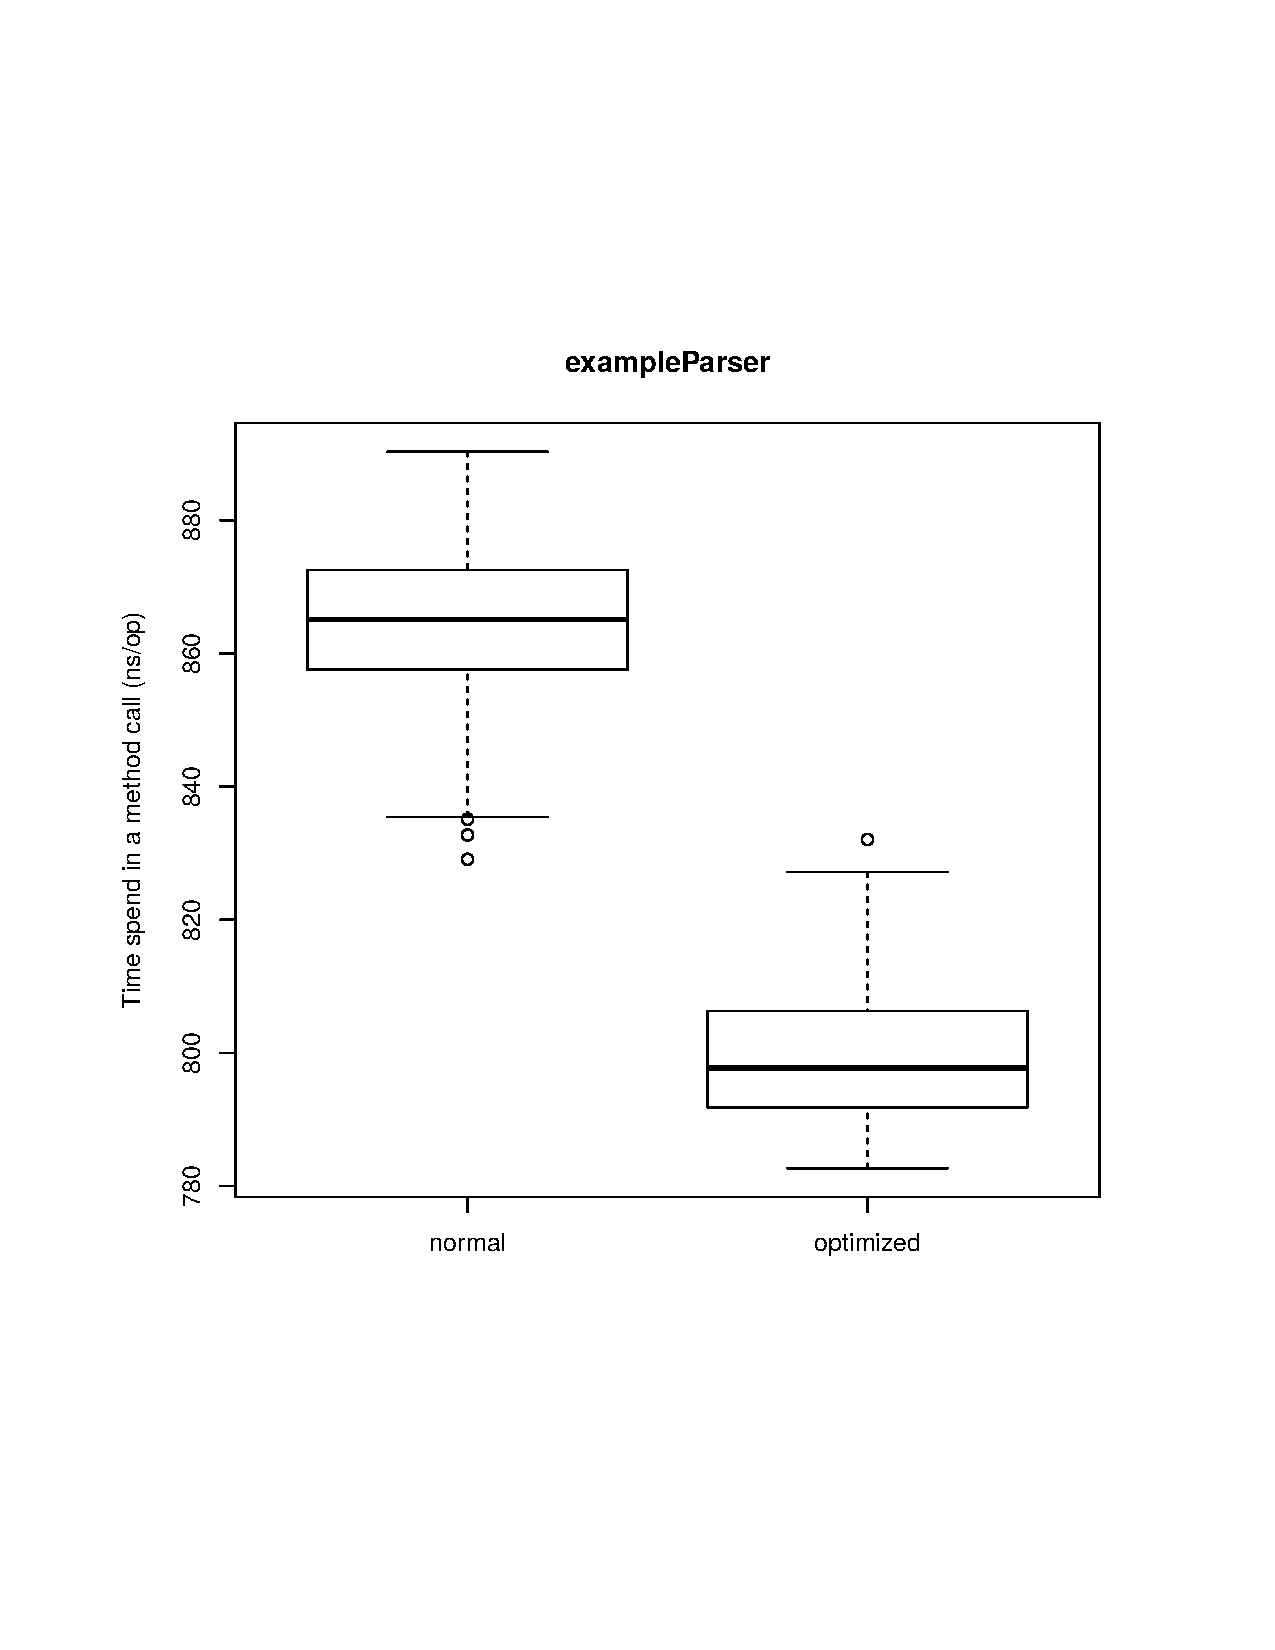
\includegraphics[trim=0mm 60mm 20mm 50mm,scale=0.50]{pictures/boxplot_exampleParser.pdf}
		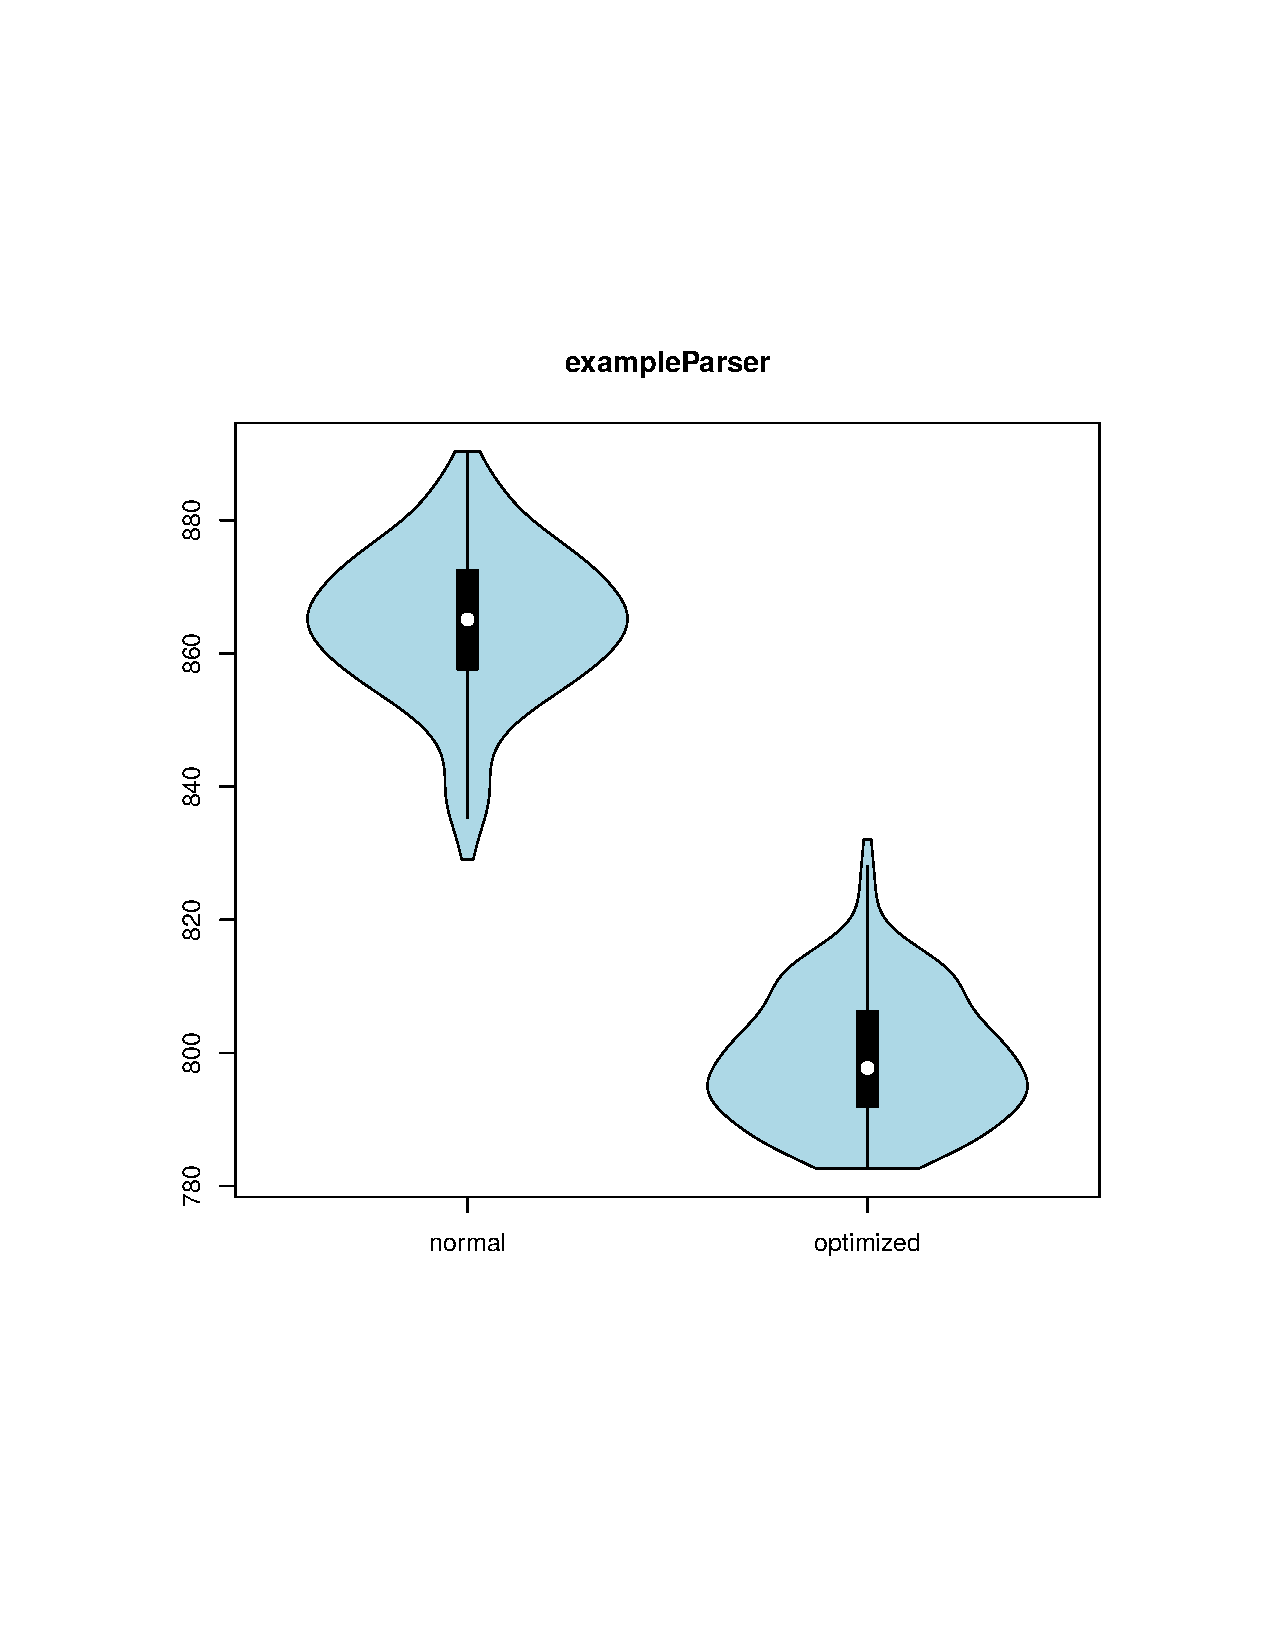
\includegraphics[trim=20mm 60mm 0mm 50mm,scale=0.50]{pictures/vioplot_exampleParser.pdf}
	}

	
	\begin{table}[H]
	\centering
		\begin{tabular}{|r|r|r|r|}
			\hline
		   	in $ns$   & Mittelwert & Median & \bf{$\pm$ $0,1\%$} \\
		 	\hline
		 	\hline
		 	normal    & 864,41 & 865,10 & 2,689 \\ 
		  	optimiert & 799,14 & 797,72 & 2,295 \\
		  	\hline
		  	
		\end{tabular}
	\end{table}

	\caption{Ergebnis des Example Parser Benchmark}\label{bp:exampleBench}
\end{figure}


\subsubsection{Auswertung}

Aufgrund der gegenseitigen Abstimmung von den beiden optimierten Typen \texttt{SubstringString} und
\texttt{StringListBuilder} können die beiden Referenzen auch ohne irgendwelche 
Konvertierungen miteinander innerhalb der Methode koexistieren. Dies führt dazu, dass
erstellte \texttt{SubstringString} Referenzen direkt dem optimierten \texttt{StringBuilder} übergeben
werden können. 

Dieser Benchmark soll zeigen, dass eine Optimierung, wenn auch für eine eigens dafür 
entwickelte Methode, möglich ist. In den folgenden Benchmarks werden realitätsnahe Methoden für 
den Test des Systems verwendet.
 
\subsection{Xalan}

Zur Auswertung des Systems wurde der freie XSLT-Prozessor \textit{XALAN} verwendet. Dieser lag in Form 
eines Java Archivs vor, das aus dem Quellcode der Version 2.7.2 gebaut wurde. 

Um geeignete Methoden für die Benchmarks zu finden, wurden die Anzahl der \texttt{substring(..)}
Aufrufe pro \texttt{*.java} Datei gezählt und diese Kandidaten nach absteigender Anzahl sortiert.
In den Kandidaten wurden diejenigen vier Methoden als Tests verwendet, welche die meisten 
Aufrufe von \texttt{substring} innerhalb der Methode besaßen. So fiel die Wahl auf die folgenden 
Methoden:

\begin{description}
	\item [\texttt{org.apache.xalan.xsltc.runtime.BasisLibrary.checkAttribQName(String)}]
		prüft ob der gegebene XML-Attribut Name syntaktisch valide ist.
	\item [\texttt{org.apache.xml.utils.URI.new(java.lang.String)}]
		erzeugt ein neues URI Objekt. 
	\item [\texttt{org.apache.xpath.objects.XNumber.str()}]
		erstellt eine String Repräsentation des XNumber Objekts.
	\item [\texttt{javax.xml.xpath.XPath.compile(java.lang.String)}]
		kompiliert den gegebenen XPath Ausdruck in ein auswertbares XPath-Objekt.
		
		Die eigentlich identifizierte Methode ist \texttt{tokenize} des verwendeten 
		Lexers. Da dieser aber die Sichtbarkeit package-private
		besitzt, wurde der kompletter Use Case, in dem der Lexer verwendet wird, 
		für die Auswertung benutzt.
\end{description}

Als Eingaben dienten Werte, die der im Projekt enthaltenen Beispiel XML Dateien entnommen wurden, 
und daher einen möglichst realen Ausführungskontext darstellen.

\subsubsection{checkAttribQName}

Diese Funktion prüft die syntaktische Validität eines XSLT-Attribut Namens. Der Name anhand 
der ersten beiden ':' getrennt, was mit Hilfe der \texttt{substring} Methode geschieht. 

Aufgerufen wurde diese Methode mit dem Wert 'xmlns:redirect'. Die folgende Abbildung zeigt 
die Ergebnisse der Messung.

\begin{figure}[H]
	\centering

	\centerline{
		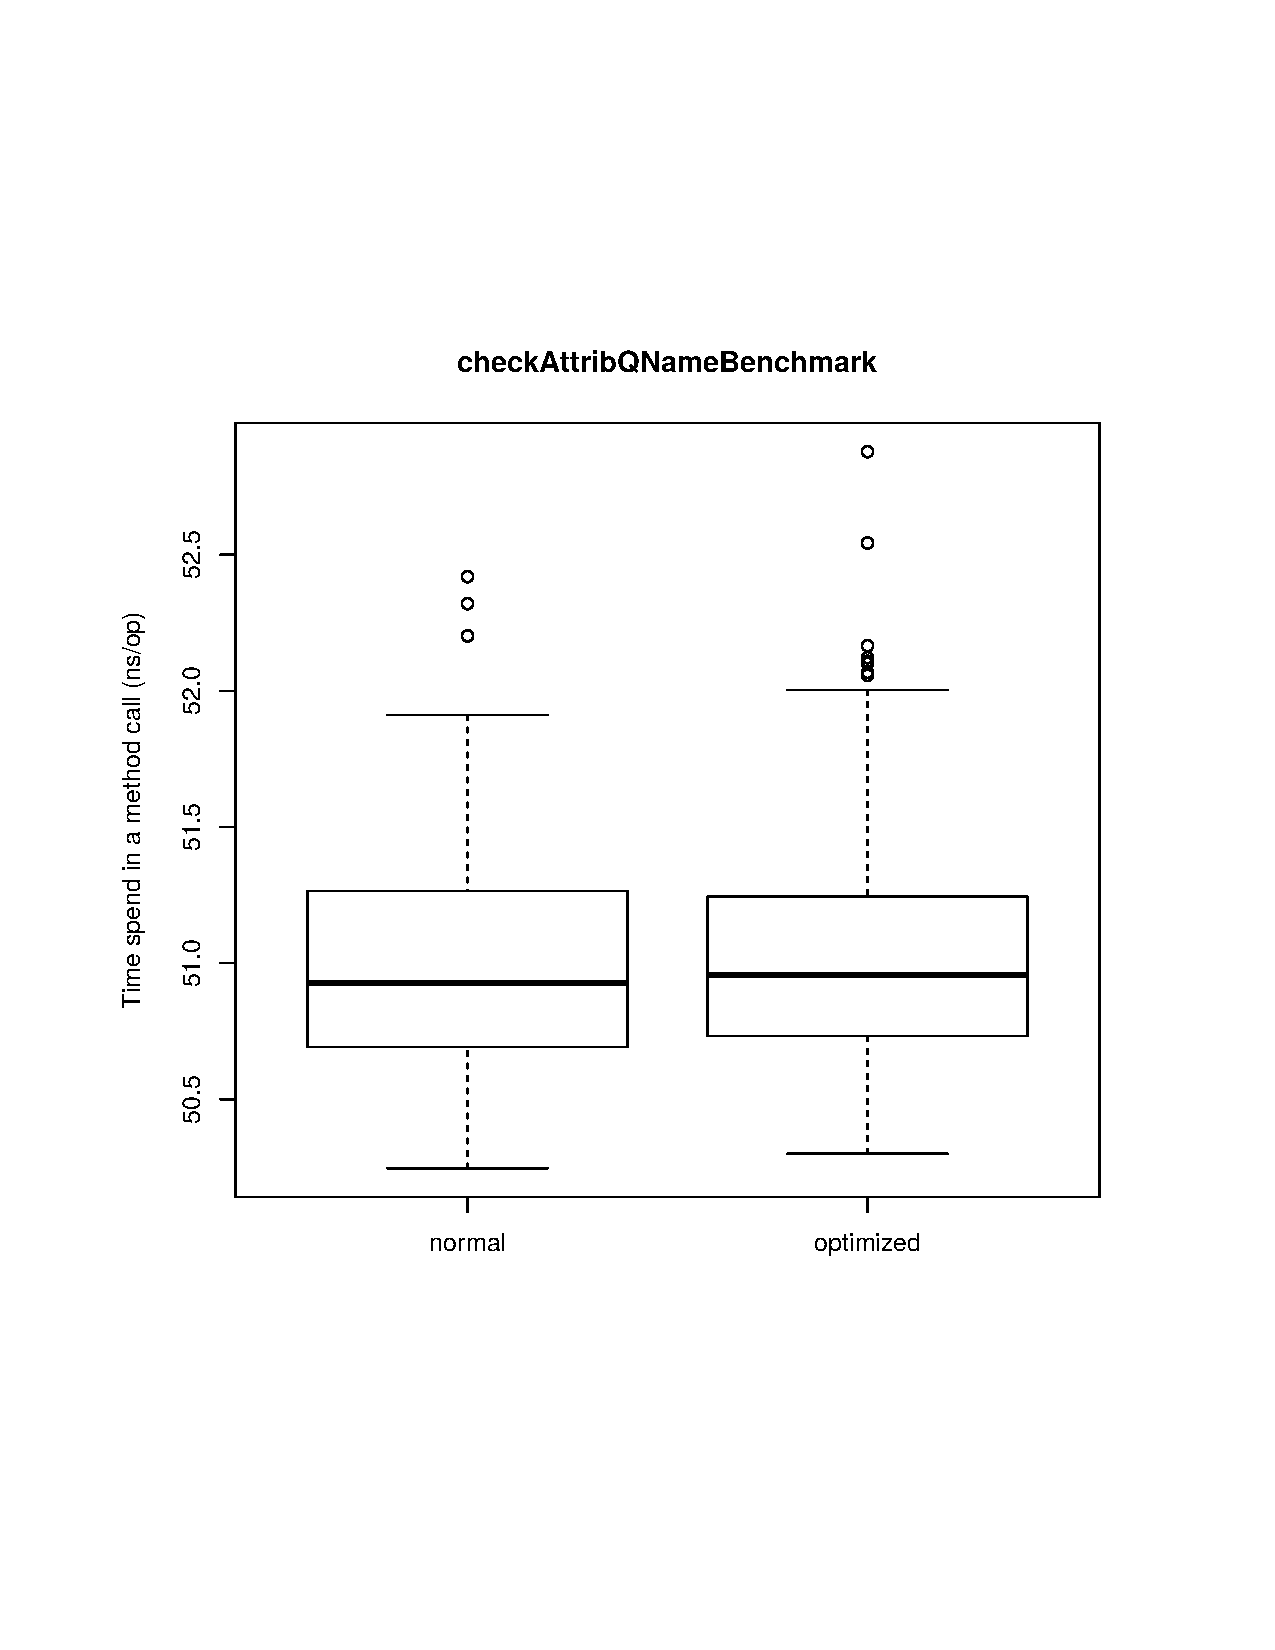
\includegraphics[trim=0mm 60mm 20mm 50mm,scale=0.50]{pictures/boxplot_checkAttribQName.pdf}
		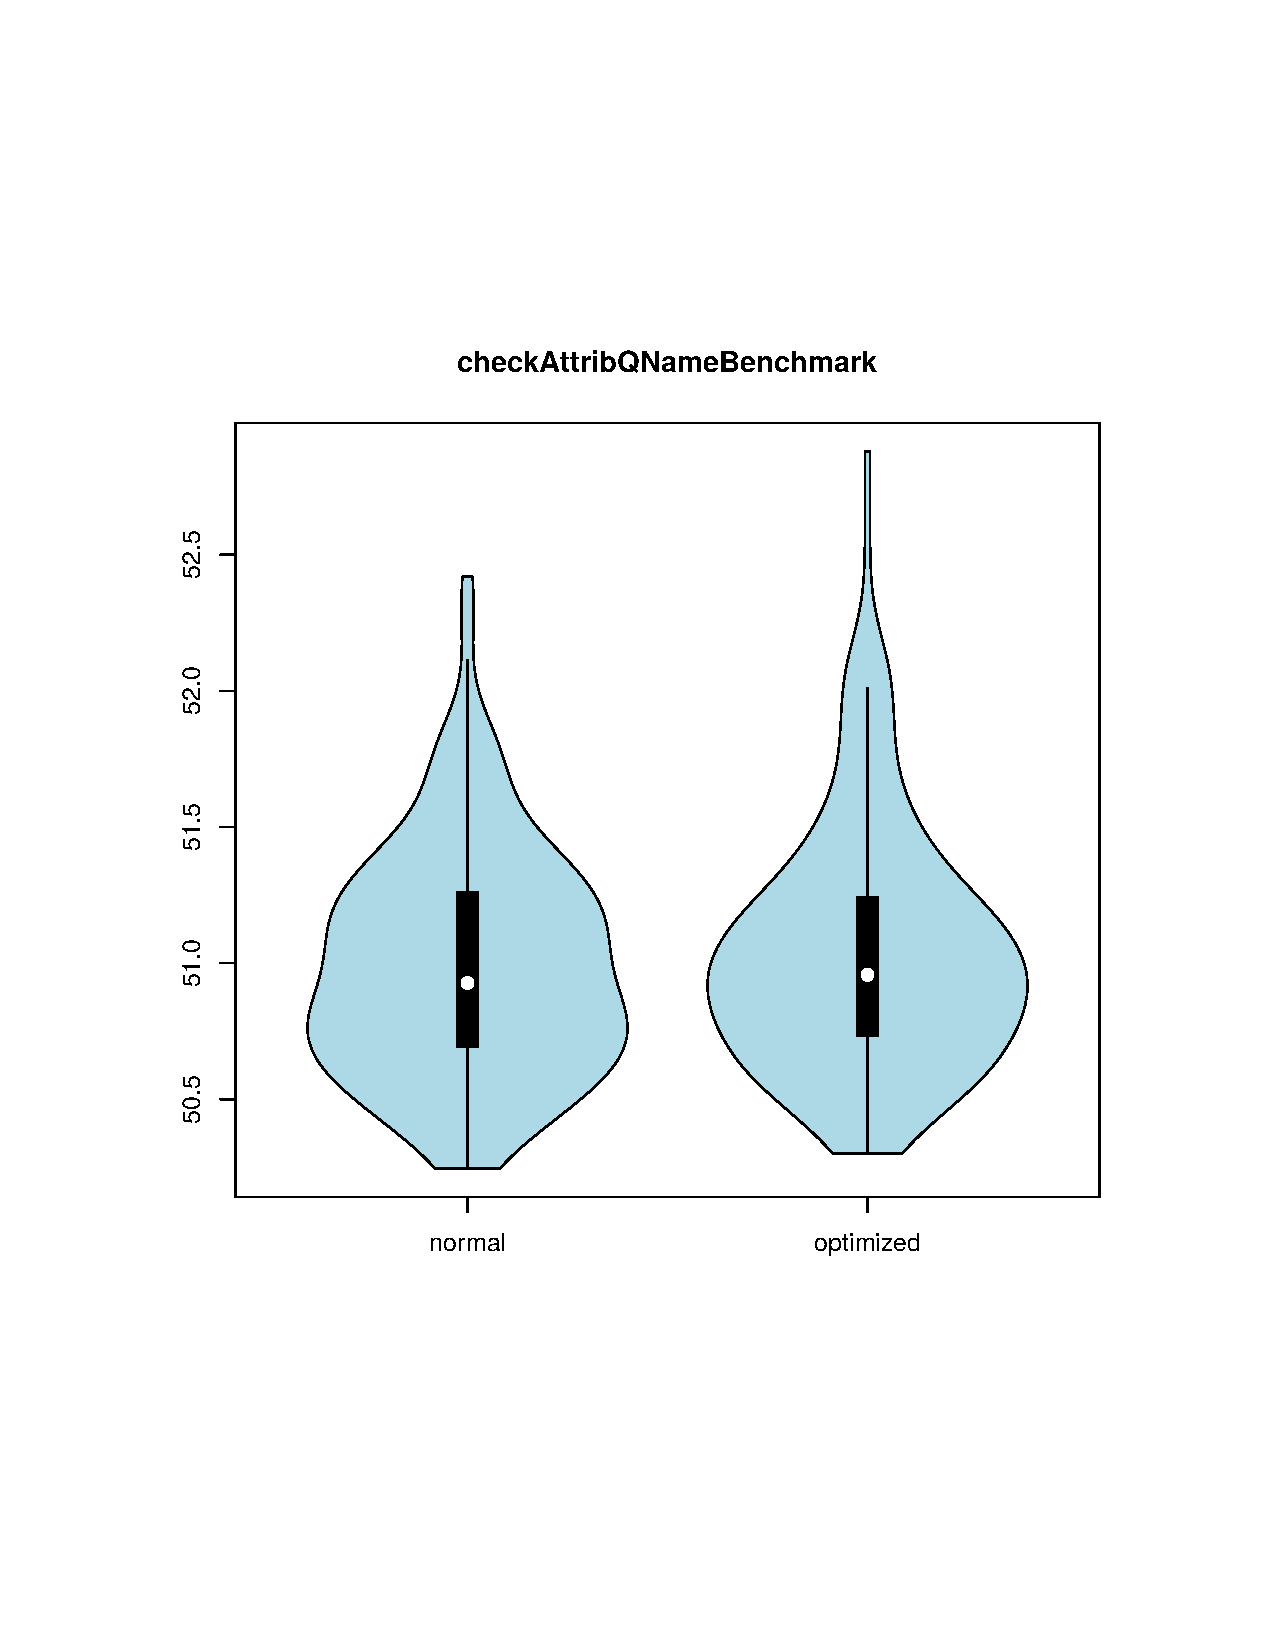
\includegraphics[trim=20mm 60mm 0mm 50mm,scale=0.50]{pictures/vioplot_checkAttribQName.pdf}
	}

	\begin{table}[H]
	\centering
		\begin{tabular}{|r|r|r|r|}
			\hline
		   	in $ns$  & Mittelwert & Median & \bf{$\pm$ $0,1\%$} \\
		 	\hline
		 	\hline
		  	normal & 50,99 & 50,92 & 0,104 \\
		 	optimiert & 51,03 & 50,96 & 0,108 \\ 
		  	\hline
		  	
		\end{tabular}
	\end{table}

	\caption{Ergebnis des checkAttribQName Benchmark}\label{bp:checkAttrBench}
\end{figure}

\paragraph{Auswertung}

Die optimierte Referenz wird als Parameter an die Methode übergeben. Also beginnt mit diesem 
Parameter-Knoten die Bubble für diese Referenz wird somit zu Beginn der Methode in einen
optimierten \texttt{SubstringString} konvertiert. Allerdings werden in den folgenden beiden 
Zeilen die Positionen der Doppelpunkte des Strings ermittelt. Die Methoden
werden aber nicht von dem optimierten Typ angeboten, was dazu führt, dass an beiden dieser 
Stellen eine Rückkonvertierung zum originalen Typ stattfinden muss. 

Dieser zusätzliche Aufwand sorgt dafür, dass die Optimierung des \texttt{substring} Aufrufs
durch die Konvertierungen wieder ausgeglichen wird. 

\subsubsection{instantiateURI}

Bei dieser Methode handelt es sich um den Konstruktor der Klasse\\ \texttt{org.apache.xml.utils.URI}.
Der erwartet einen String, der die zu repräsentierende URI enthält. Der Konstruktor teilt
die übergebene Zeichenkette in semantische Bausteine, wie das Protokoll, die Domain oder den Pfad.
Zu diesem wird die Methode \texttt{substring} wiederholt auf der übergebenen Zeichenkette angewendet. 

Die Messung wurde mit dem Wert 'http://xml.apache.org/xalan-j/apidocs/
javax/xml/transform/package-summary.html' durchgeführt. Die folgende Abbildung präsentiert 
die Ergebnisse dieses Benchmarks.

\begin{figure}[H]
	\centering
	
	\centerline{
		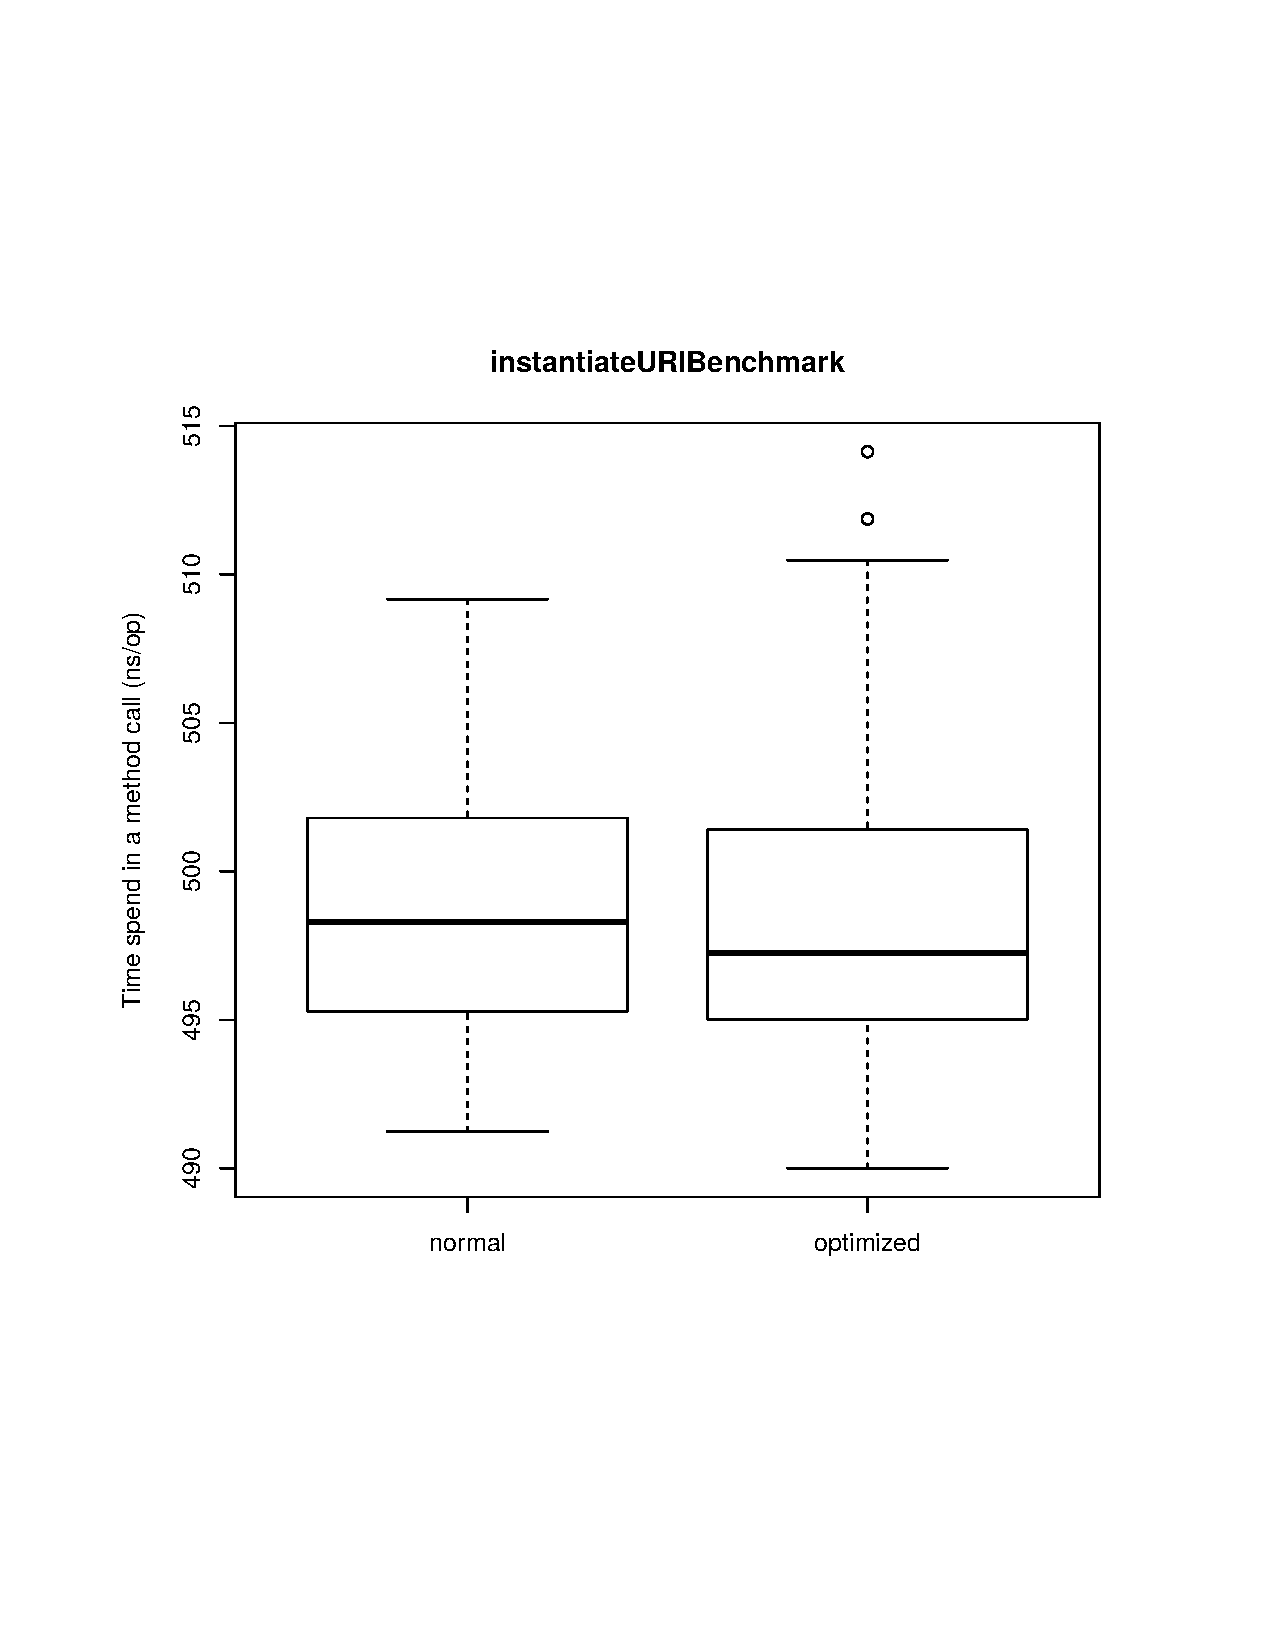
\includegraphics[trim=0mm 60mm 20mm 50mm,scale=0.50]{pictures/boxplot_instantiateURI.pdf}
		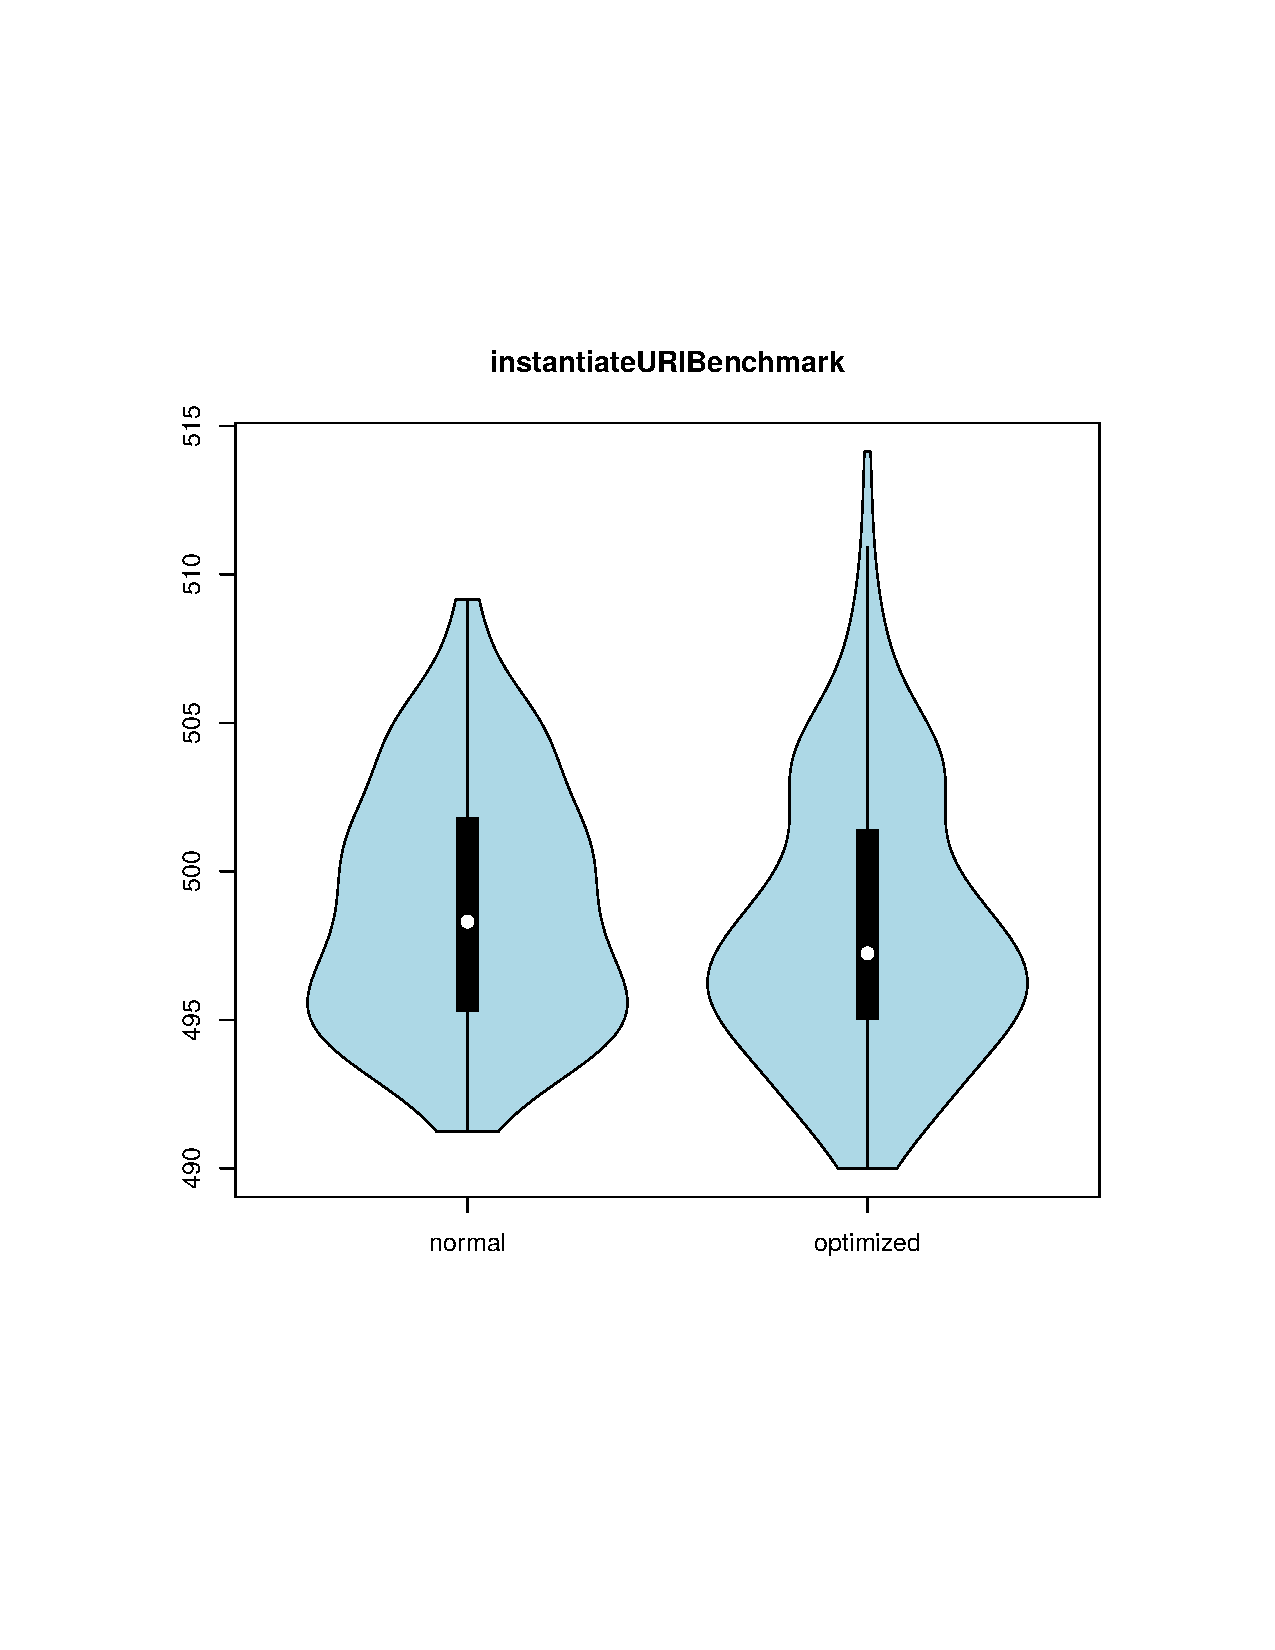
\includegraphics[trim=20mm 60mm 0mm 50mm,scale=0.50]{pictures/vioplot_instantiateURI.pdf}
	}

	\begin{table}[H]
	\centering
		\begin{tabular}{|r|r|r|r|}
			\hline
		   	in $ns$  & Mittelwert & Median & \bf{$\pm$ $0,1\%$} \\
		 	\hline
		 	\hline
		  	normal 	  & 498,79 & 498,30 & 0,965 \\
		 	optimiert & 498,22 & 497,24 & 1.086 \\ 
		  	\hline
		  	
		\end{tabular}
	\end{table}

	\caption{Ergebnis des instantiateURI Benchmarks}\label{bp:instURIBench}
\end{figure}

\paragraph{Auswertung}

Bei der Optimierung dieser Methode stellen sich einige Probleme dar. Die zur 
Optimierung verwendete Referenz wird durch einen \texttt{trim()} Aufruf auf der
übergebenen URI definiert. Diese Referenz wird innerhalb der Methode häufig benutzt,
und mit jedem \texttt{substring} Aufruf auf diese Referenz wird eben diese wieder 
überschrieben. Zu den sonstigen aufgerufenen Methoden auf diesen Referenzen gehören:

\begin{itemize}
  	\item \texttt{startsWith(String)}
  	\item \texttt{length()}
  	\item \texttt{charAt(int)} 
\end{itemize}  

Wobei der Typ \texttt{SubstringString} \texttt{length} und \texttt{charAt} 
implementiert. Darüber hinaus werden diese \texttt{SubstringString} Referenzen
an die folgenden privaten Methoden übergeben. 

\begin{itemize}
 	\item \texttt{initializeScheme(String)}
 	\item \texttt{initializeAuthority(String)}
 	\item \texttt{initializePath(String)}
\end{itemize} 

In diesen Methoden werden wiederum unter anderem \texttt{substring} Aufrufe auf 
den übergebenen String ausgeführt.

All diese anderweitigen Verwendungen der optimierten Referenz sorgen dafür, dass die
Bubble an diesen Stellen endet und eine Konvertierung zum originalen Typ 
\texttt{java.lang.String} stattfindet. Diese Konvertierungen haben allerdings negative 
Auswirkungen auf die Laufzeit, wodurch die Optimierungseffekte wieder aufgehoben werden.    

\subsubsection{xNumberToString}

Eine \texttt{org.apache.xpath.objects.XNumber} repräsentiert eine Zahl innerhalb eines
XPath Ausdrucks. Die Methode \texttt{str():java.lang.String} wandelt die intern verwaltete
Dezimalzahl in eine String Repräsentation dieses Wertes um. Dabei wird das Ergebnis
des Ausdrucks \texttt{Double.toString(val)} einem String zugewiesen, wobei \texttt{val} 
der aktuelle Wert des Objektes ist. Dieser String wird daraufhin in ein alternatives
Dezimalzahlen Format umgewandelt: 

\begin{itemize}
 	\item Es werden 'NaN' bzw. 'Infinity' Zeichenketten erzeugt.
 	\item Bei Ganzzahlen wird das folgende '.0' abgeschnitten.
 	\item Für Zahlen mit Exponenten werden diese ausgeschrieben.
\end{itemize} 

Um die verschiedenen Teile der Verarbeitung innerhalb der Methode mit zu berücksichtigen, 
wurde der Test mit verschiedenen Eingaben durchgeführt:

\begin{itemize}
	\item Einer positiven Dezimalzahl (12,34)
	\item Einer negativen Dezimalzahl (-12,34)
	\item Einer positiven Ganzzahl (12)
	\item Einer Zahl mit negativem Exponent (0,12e-5)
\end{itemize}

Im folgenden sind die einzelnen Testergebnisse aufgeführt. Eine Auswertung der
Ergebnisse folgt den Darstellungen.


\begin{figure}[H]
	\centering

	\centerline{
		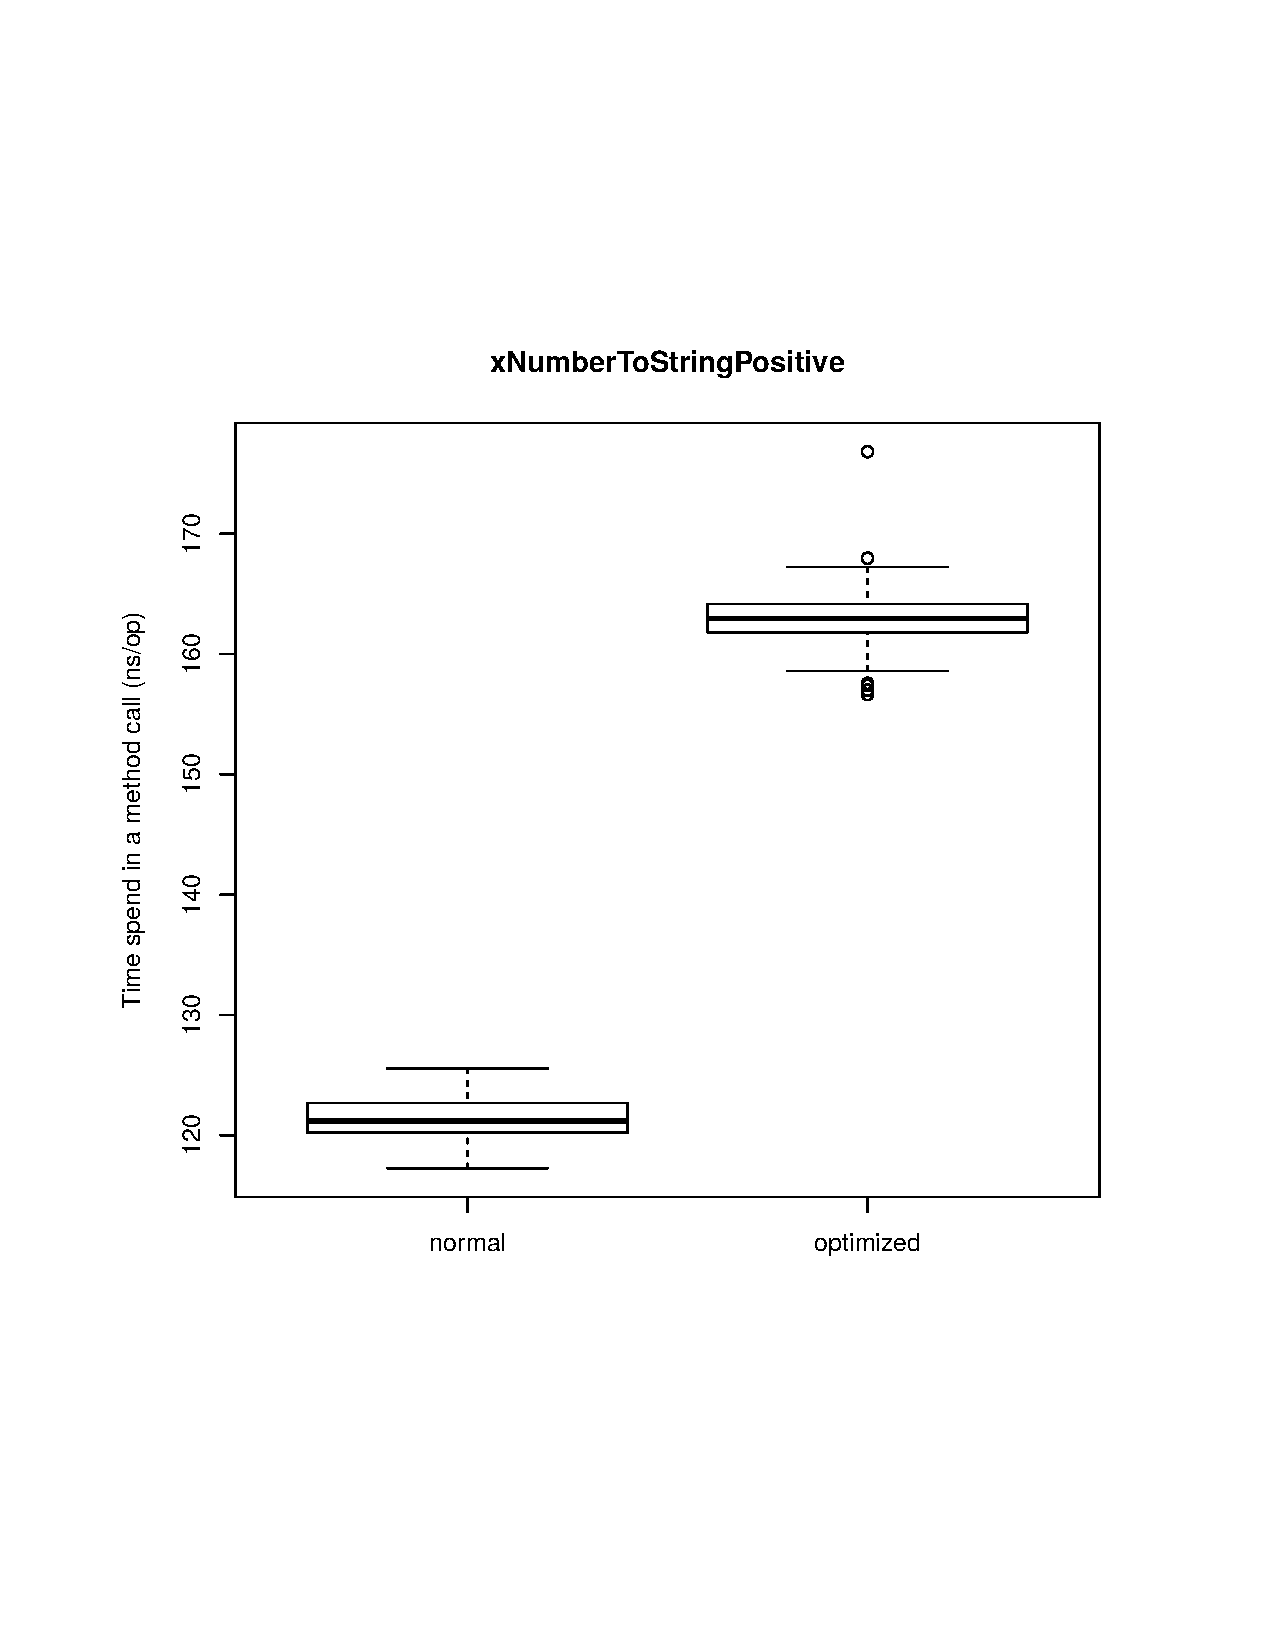
\includegraphics[trim=0mm 60mm 20mm 50mm,scale=0.50]{pictures/boxplot_xNumberToStringPositive.pdf}
		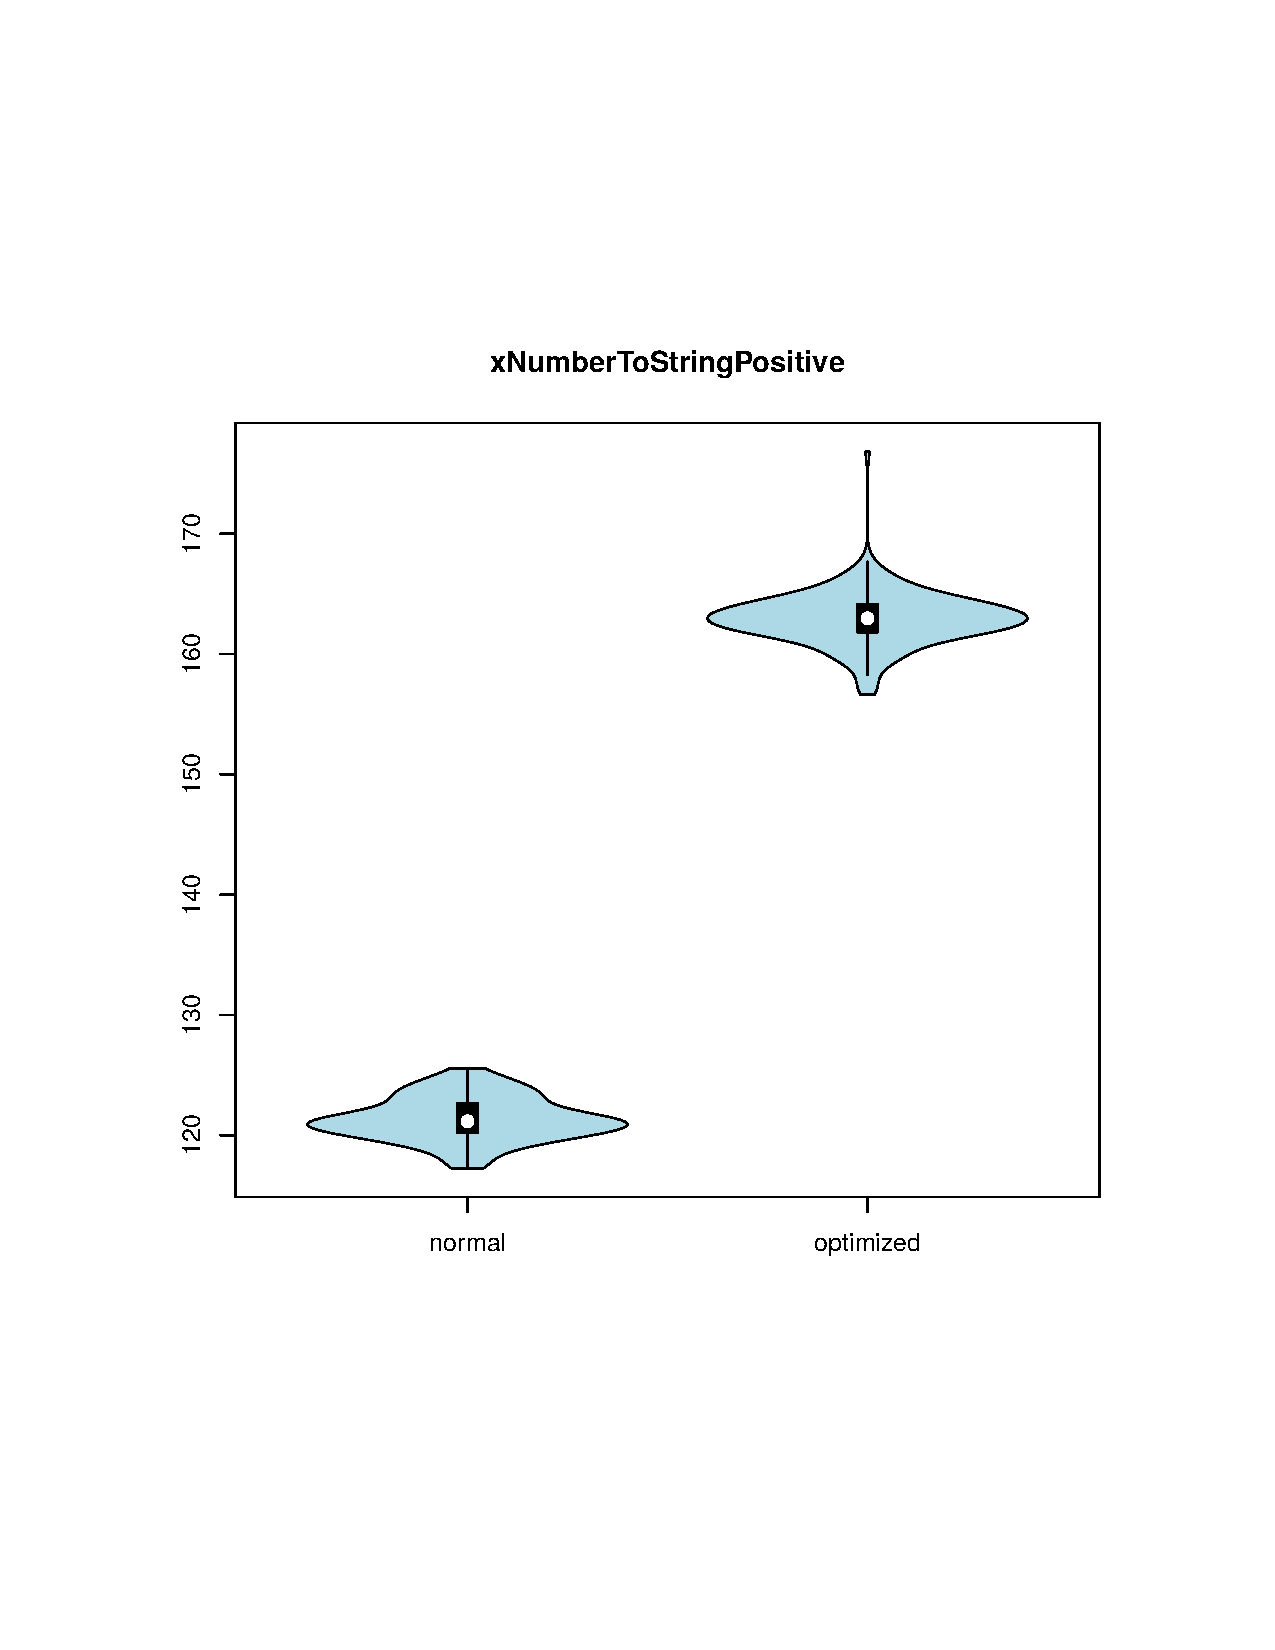
\includegraphics[trim=20mm 60mm 0mm 50mm,scale=0.50]{pictures/vioplot_xNumberToStringPositive.pdf}
	}
	\begin{table}[H]
	\centering
		\begin{tabular}{|r|r|r|r|}
			\hline
		   	in $ns$  & Mittelwert & Median & \bf{$\pm$ $0,1\%$} \\
		 	\hline
		 	\hline
		  	normal 	  & 121,38 & 121,17 & 0,425 \\
		 	optimiert & 162,93 & 162,97 & 0,518 \\ 
		  	\hline
		  	
		\end{tabular}
	\end{table}

	\caption{Ergebnis des xNumberToString Benchmarks (positive Dezimalzahl)}\label{bp:xNumPos}
\end{figure}



\begin{figure}[H]
	\centering

	\centerline{
		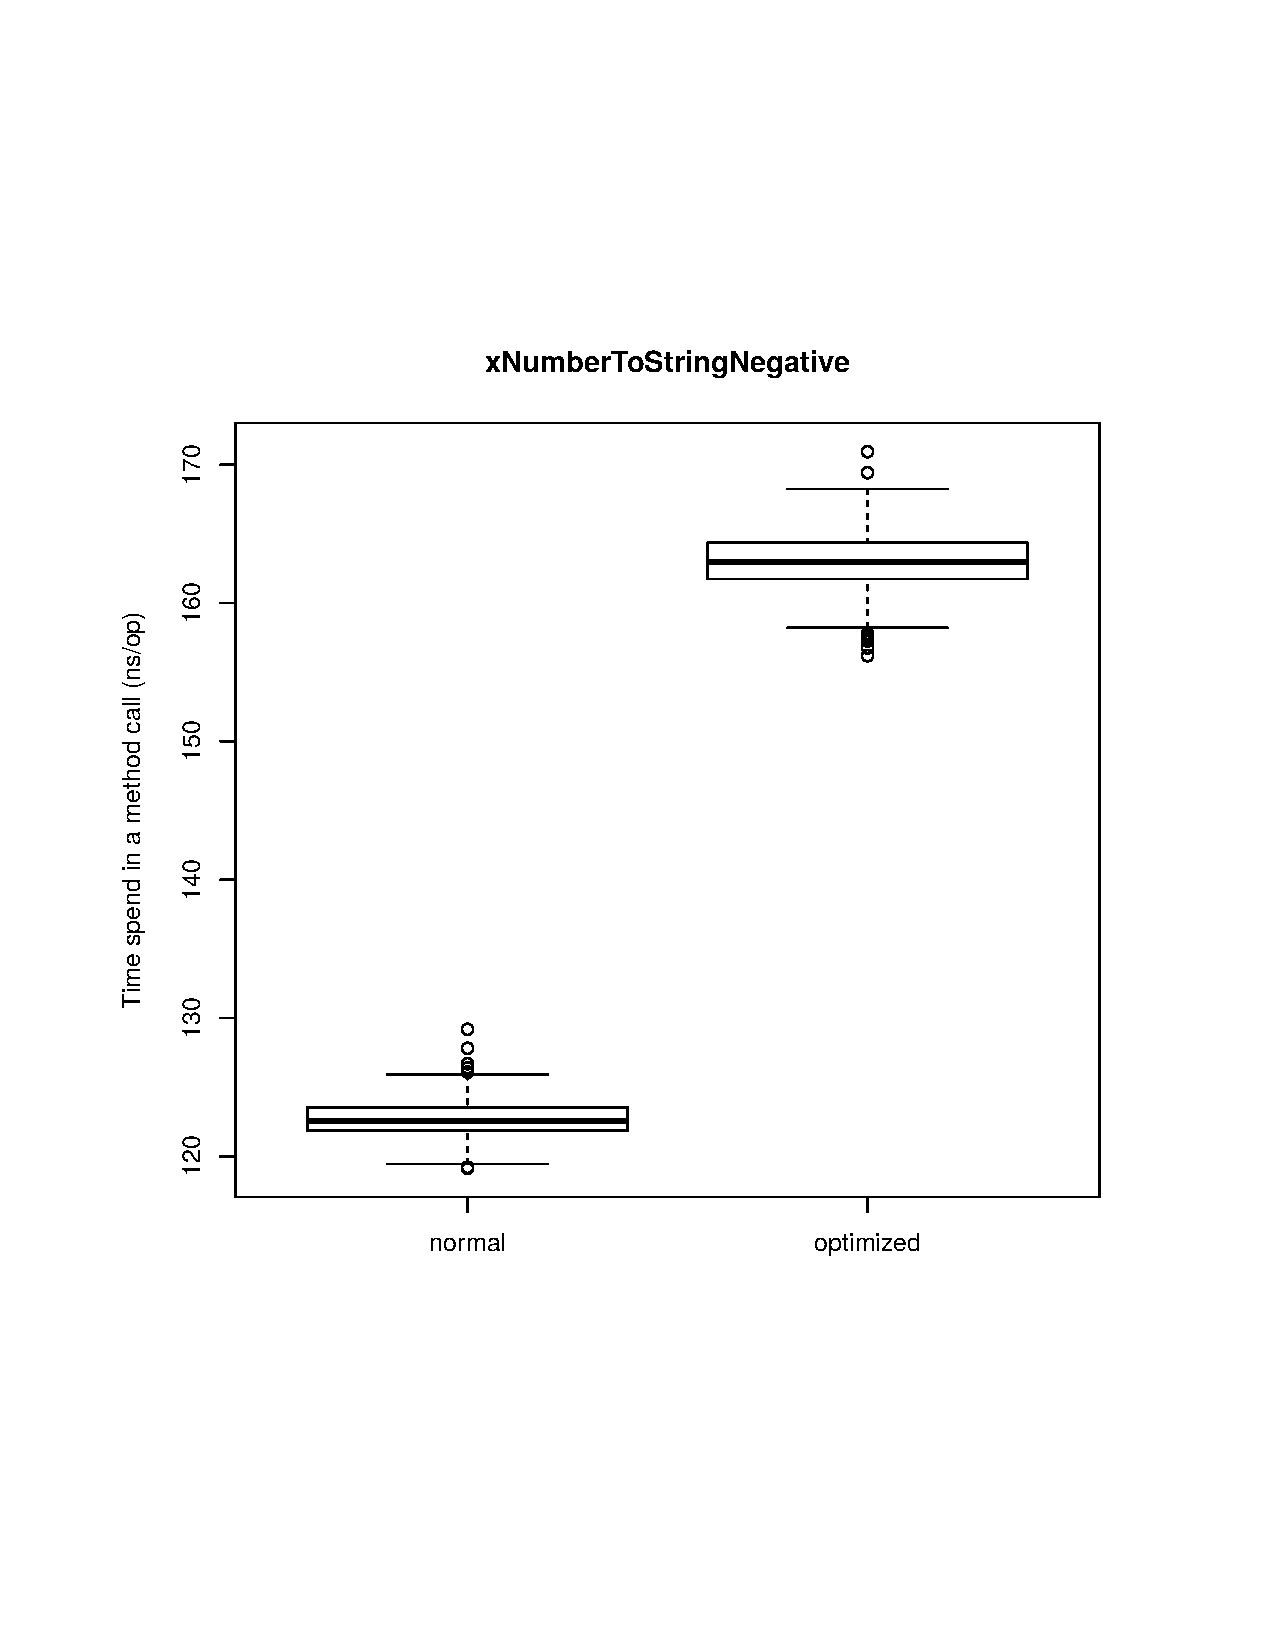
\includegraphics[trim=0mm 60mm 20mm 50mm,scale=0.50]{pictures/boxplot_xNumberToStringNegative.pdf}
		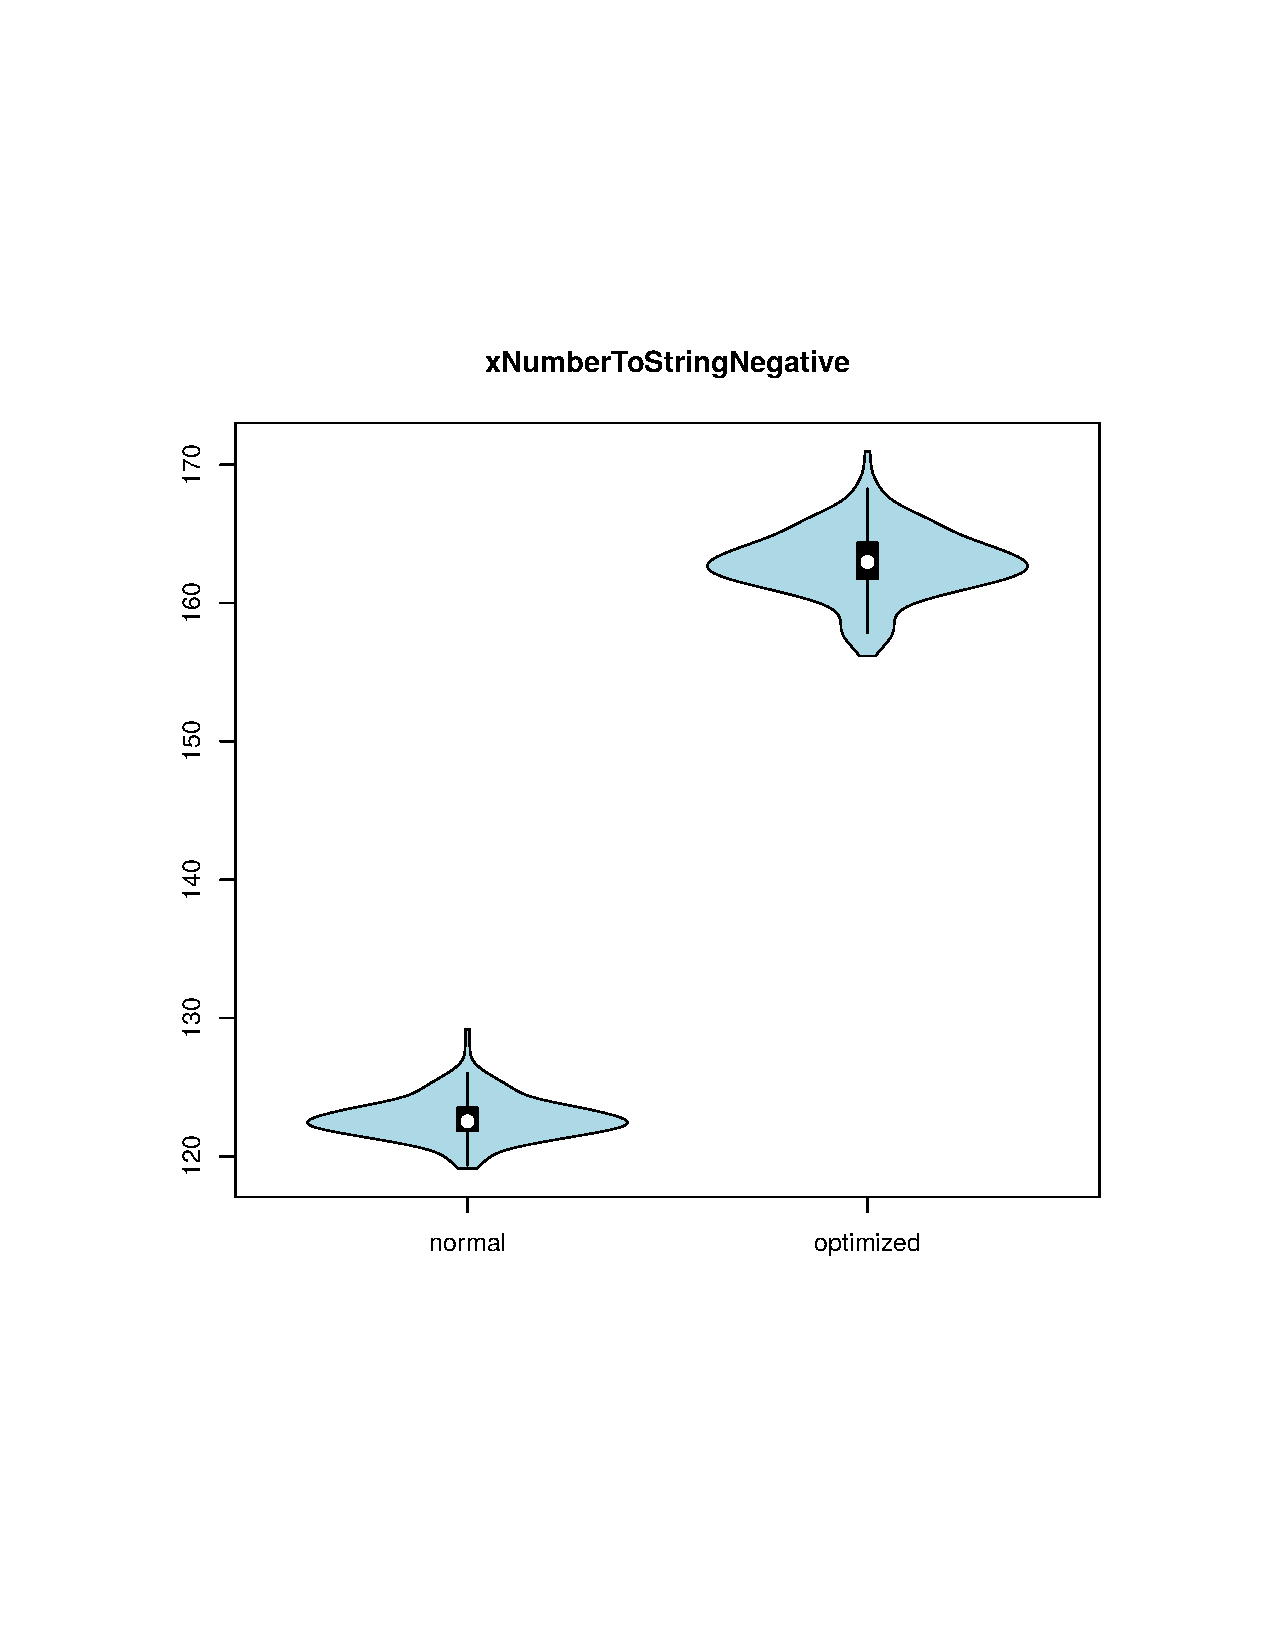
\includegraphics[trim=20mm 60mm 0mm 50mm,scale=0.50]{pictures/vioplot_xNumberToStringNegative.pdf}
	}
	\begin{table}[H]
	\centering
		\begin{tabular}{|r|r|r|r|}
			\hline
		   	in $ns$   & Mittelwert & Median & \bf{$\pm$ $0,1\%$} \\
		 	\hline
		 	\hline
		  	normal 	  & 122,78 & 122,54 & 0,359 \\
		 	optimiert & 162,91 & 162,97 & 0,572 \\ 
		  	\hline
		  	
		\end{tabular}
	\end{table}

	\caption{Ergebnis des xNumberToString Benchmarks (negative Dezimalzahl)}\label{bp:xNumNeg}
\end{figure}


\begin{figure}[H]
	\centering

	\centerline{
		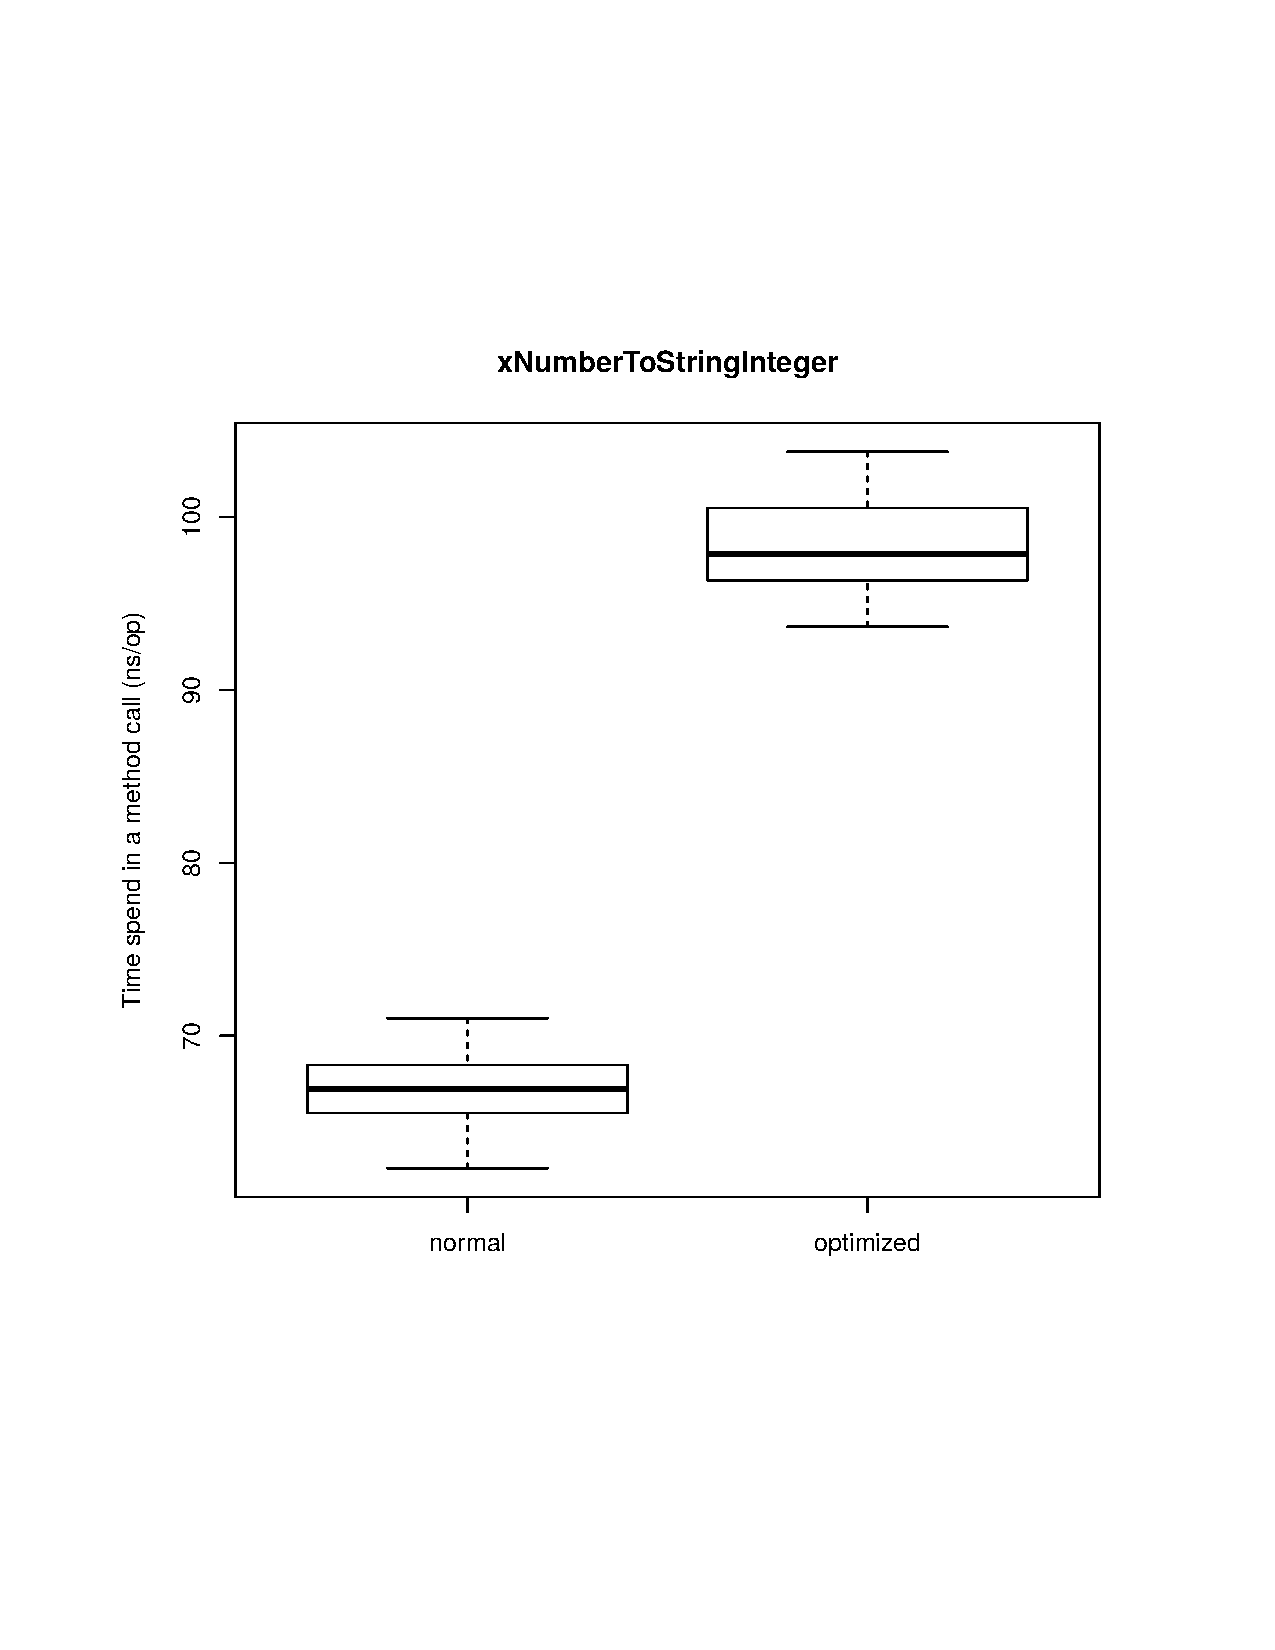
\includegraphics[trim=0mm 60mm 20mm 50mm,scale=0.50]{pictures/boxplot_xNumberToStringInteger.pdf}
		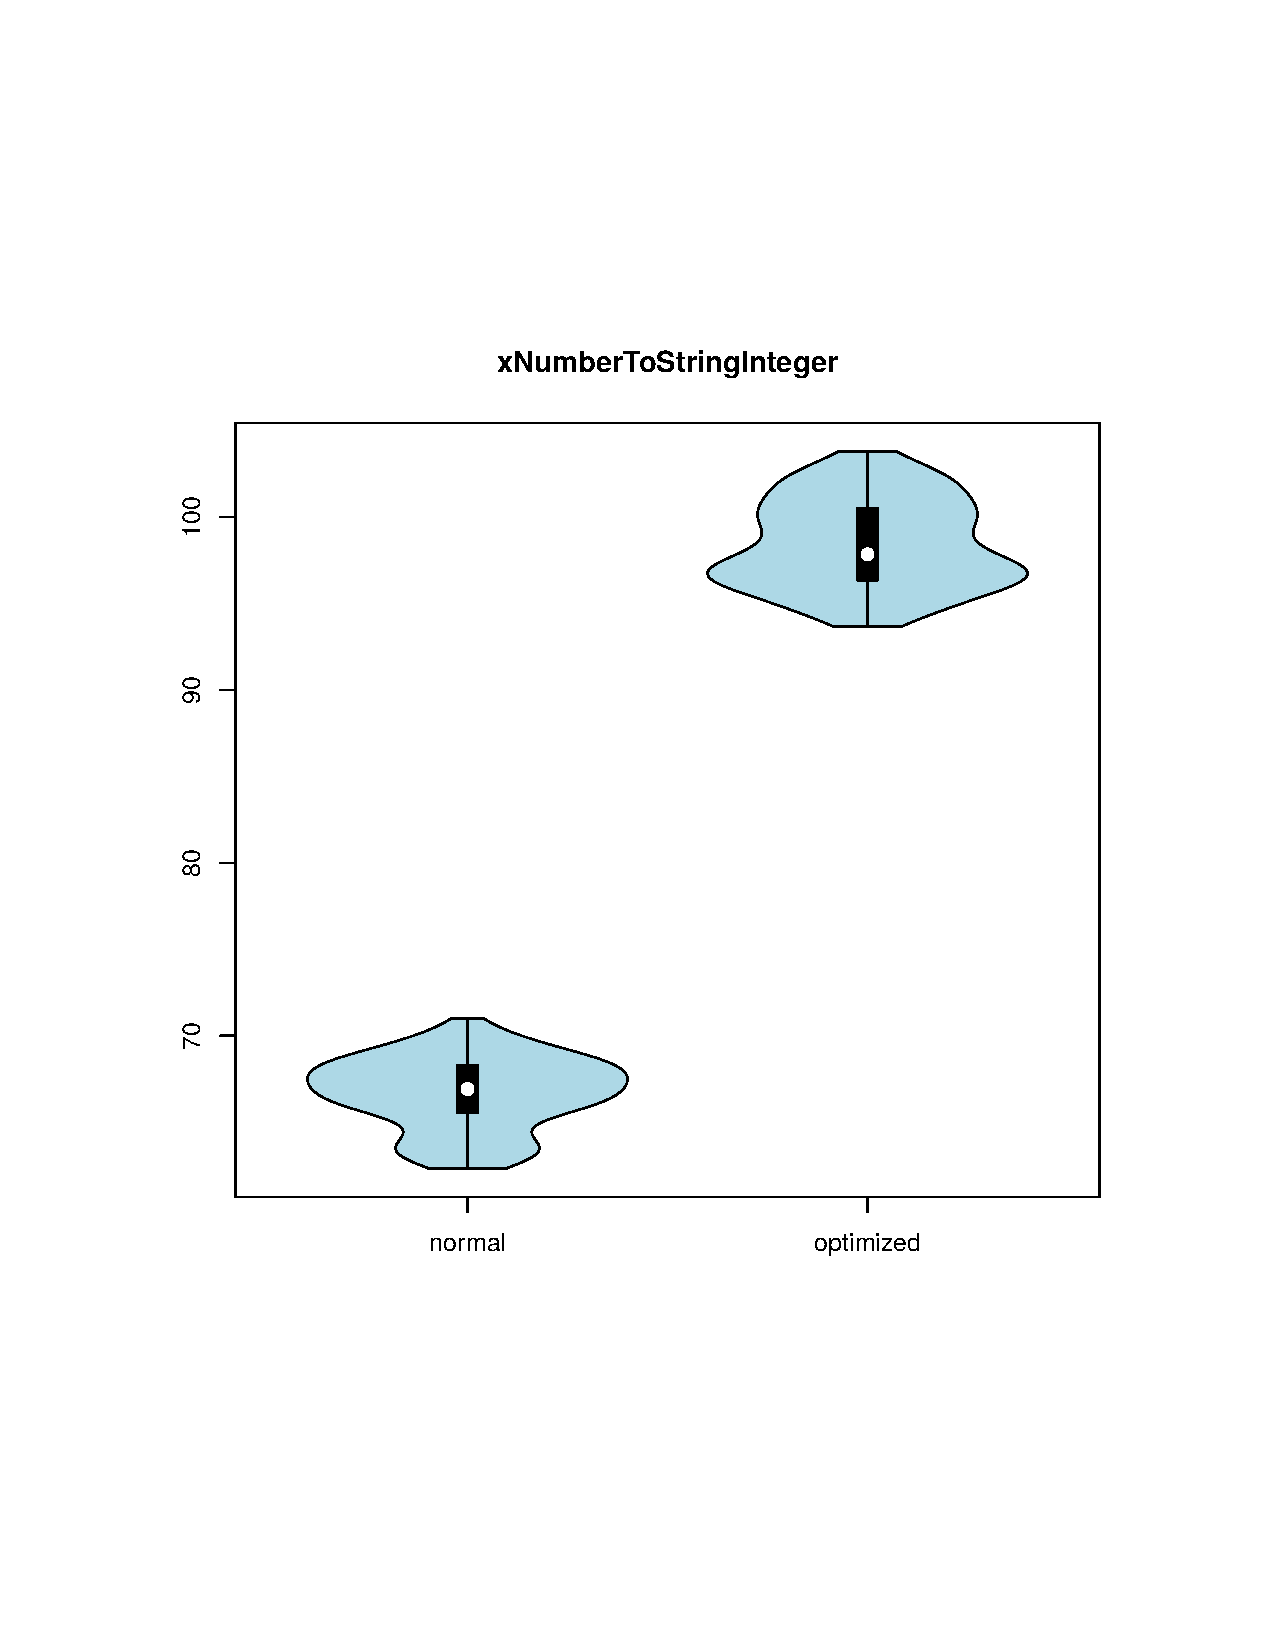
\includegraphics[trim=20mm 60mm 0mm 50mm,scale=0.50]{pictures/vioplot_xNumberToStringInteger.pdf}
	}

	\begin{table}[H]
	\centering
		\begin{tabular}{|r|r|r|r|}
			\hline
		   	in $ns$   & Mittelwert & Median & \bf{$\pm$ $0,1\%$} \\
		 	\hline
		 	\hline
		  	normal 	  & 66,69 & 66,91 & 0,488 \\
		 	optimiert & 98,42 & 97,84 & 0,605 \\ 
		  	\hline
		  	
		\end{tabular}
	\end{table}

	\caption{Ergebnis des xNumberToString Benchmarks (positive Ganzzahl)}\label{bp:xNumInt}
\end{figure}


\begin{figure}[H]
	\centering

	\centerline{
		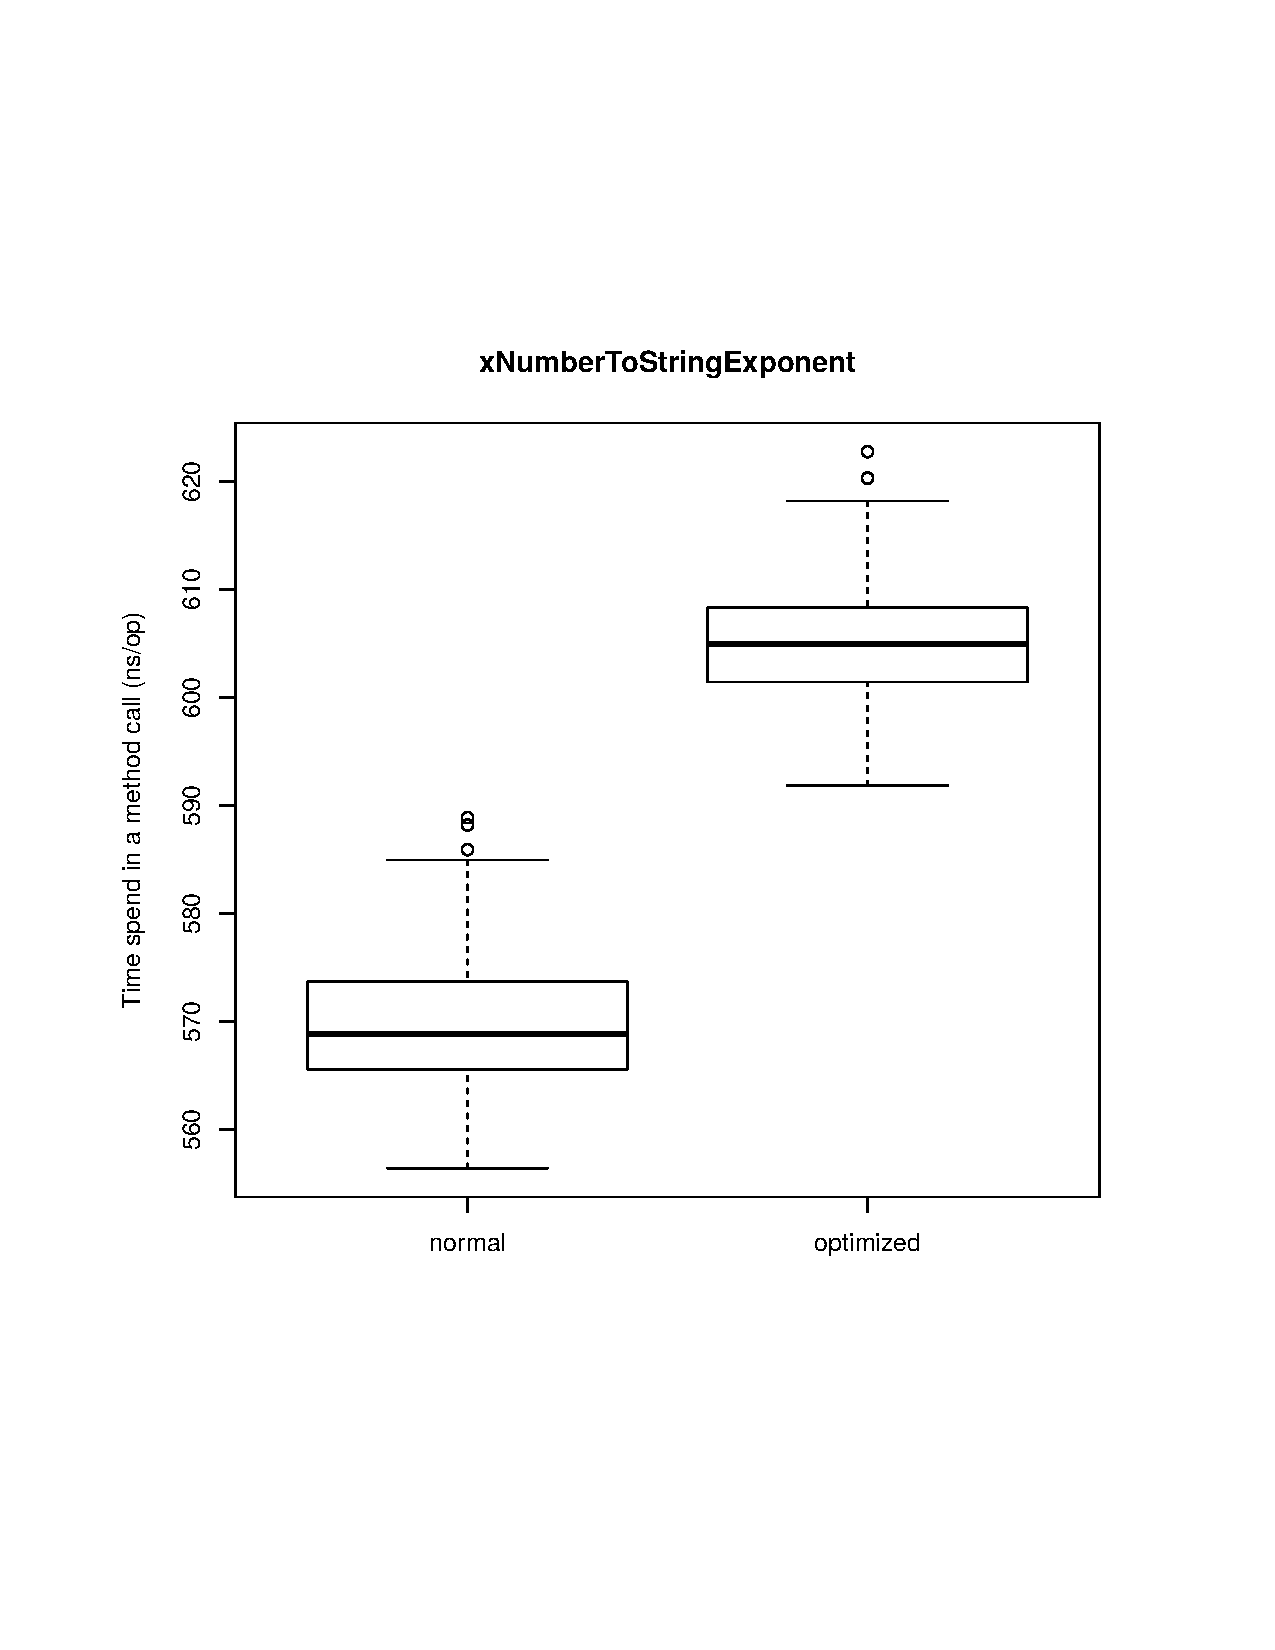
\includegraphics[trim=0mm 60mm 20mm 50mm,scale=0.50]{pictures/boxplot_xNumberToStringExponent.pdf}
		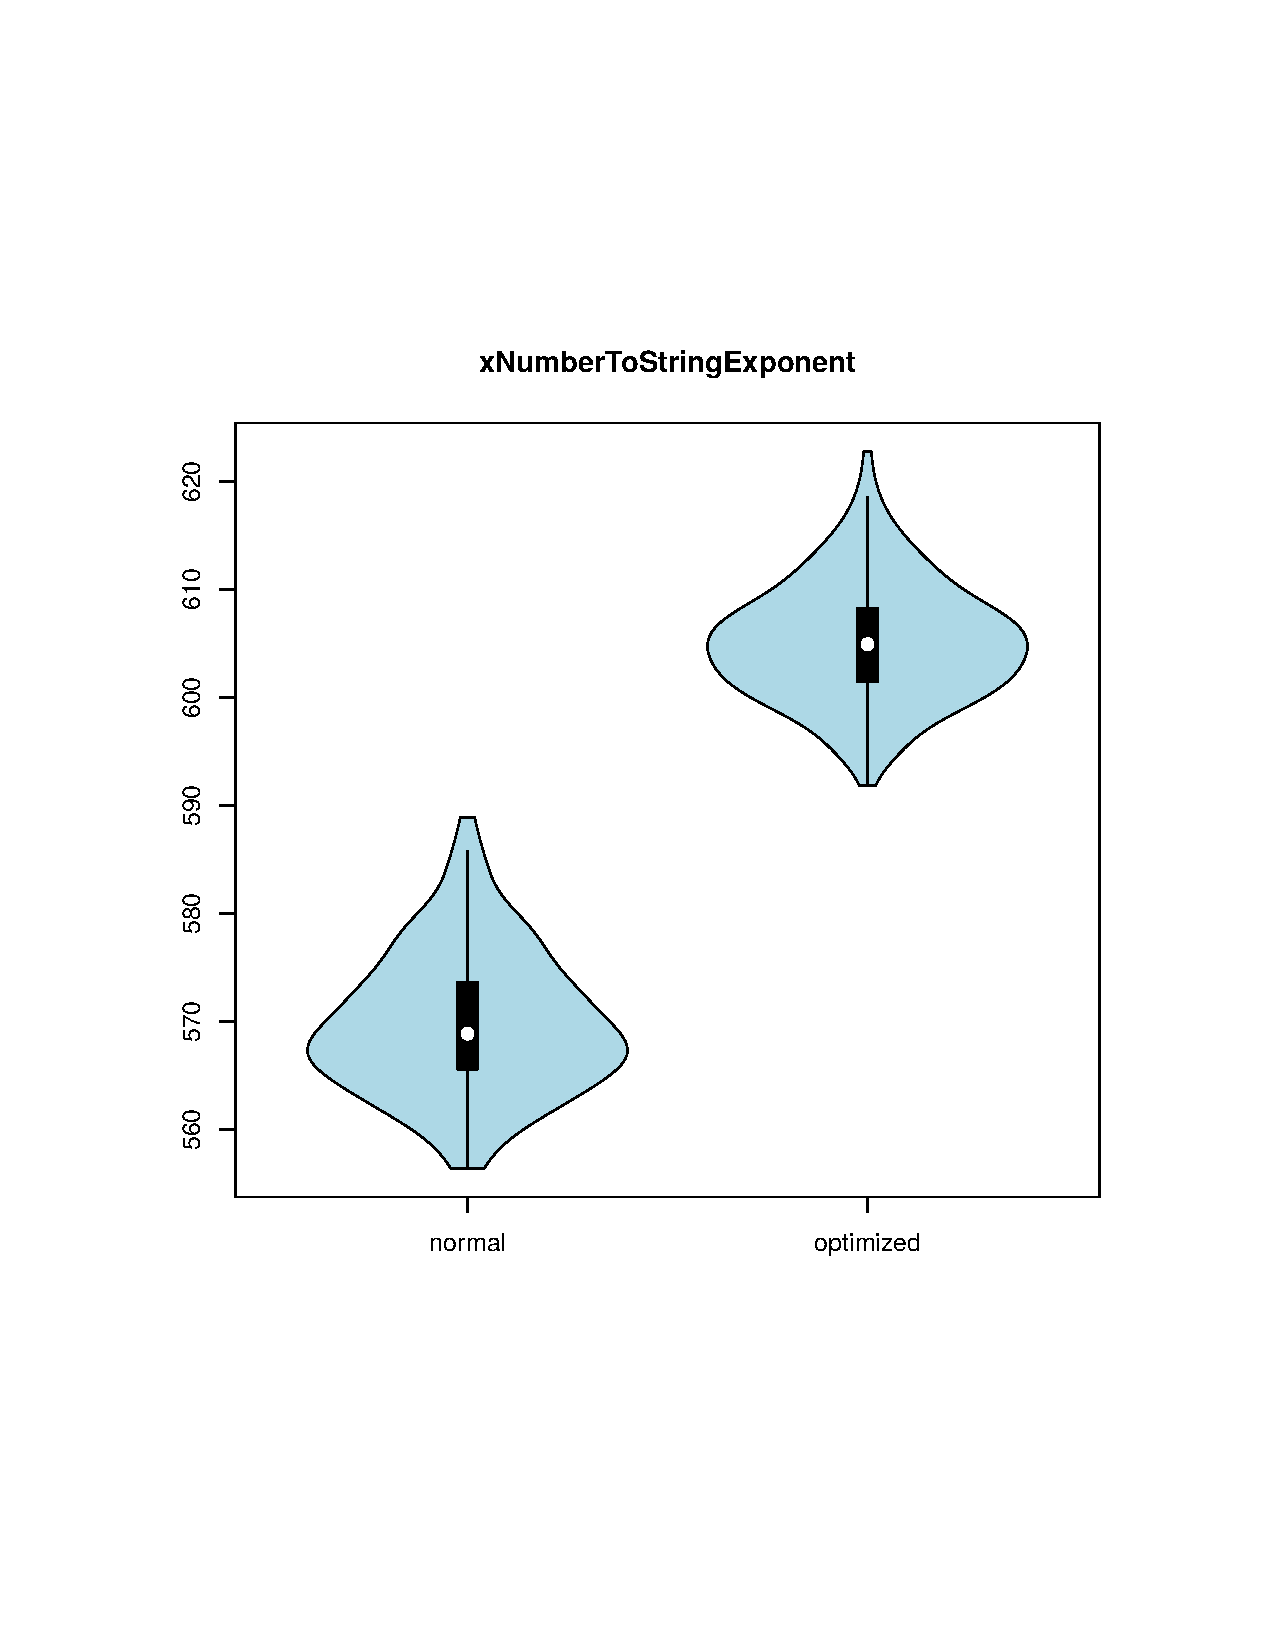
\includegraphics[trim=20mm 60mm 0mm 50mm,scale=0.50]{pictures/vioplot_xNumberToStringExponent.pdf}
	}

	\begin{table}[H]
	\centering
		\begin{tabular}{|r|r|r|r|}
			\hline
		   	in $ns$   & Mittelwert & Median & \bf{$\pm$ $0,1\%$} \\
		 	\hline
		 	\hline
		  	normal 	  & 569,85 & 568,86 & 1.530 \\
		 	optimiert & 605,16 & 604,93 & 1,291 \\ 
		  	\hline
		  	
		\end{tabular}
	\end{table}

	\caption{Ergebnis des xNumberToString Benchmarks (Zahl mit negativem Exponent)}\label{bp:xNumExp}
\end{figure}

\paragraph{Auswertung}

Die \texttt{xNumberToString} Methode erzeugt eine \texttt{String} Repräsentation der
im Objekt verwalteten Gleitkommazahl. Der Wert ist vom Typ \texttt{double}. Der 
\texttt{String} wird über einen Aufruf von \texttt{Double.toString(double)} erzeugt, dem der 
\texttt{double} Wert der Klassen Eigenschaft übergeben wird. Die \texttt{String} Referenz wird innerhalb der 
Methode formatiert. Dies geschieht über Kontrollflüsse, die abhängig von der ursprünglichen Zahl sind.
Die vier vorgestellten Benchmarks decken die verschiedenen Verarbeitungsschritte ab. Die auf der
Referenz in jedem Fall aufgerufenen Methoden (abgesehen von \texttt{substring}) sind:

\begin{itemize}
	\item \texttt{length()}
	\item \texttt{charAt(int)}
	\item \texttt{indexOf(char)}
\end{itemize}

Die Methode \texttt{indexOf(char)} wird nicht von dem optimierten Typ unterstützt.
Da der Aufruf allerdings für jede Zahl $\neq 0$ aufgerufen wird (es wird nach dem '\texttt{e}' in
Exponenten gesucht), muss jeder \texttt{SubstringString} vor dem Aufruf in einen String
konvertiert werden. 

Diese Konvertierungen für den Aufruf von \texttt{indexOf}, zum Beginn und zum Ende der Methode, 
führen zu einer beträchtlichen Anstieg der Laufzeit in der optimierten Variante dieser Methode.


\subsubsection{compileXPath}

Ein XPath Ausdruck (XML Path Language) stellt eine Abfrage gegen einen XML-Baum dar. Die Sprache
ist ein Standard des W3C und stellt einen wichtigen Baustein bei der XML Transformation dar.
Xalan bietet eine API, die es ermöglicht XPath Abfragen auf DOM-Bäume auszuführen. Teil dieser
API ist es, einen gegebenen String in eine ausführbare Objektstruktur umzuwandeln. Zu diesem Zweck
wird der gegebene \texttt{String} zunächst von einem Lexer in einzelne Token geteilt, die verwendet werden,
um den abstrakten Syntax Baum des Ausdrucks zu erstellen.

Die Methode \texttt{org.apache.xpath.compiler.Lexer.tokenize(String, \\Vector)} führt das Zerteilen 
des Eingabe-Strings in einzelne Token durch. Dieser Benchmark kompiliert den XPath Ausdruck
'\texttt{ex:addFunc(2, 3) + \$xyz}' indem die Methode \texttt{javax.xml.xpath.XPath.compile(String)}
mit dem entsprechenden \texttt{String} aufgerufen wird. Abbildung \ref{bp:compile} zeigt die Ergebnisse 
der Messung.

\begin{figure}[H]
	\centering

	\centerline{
		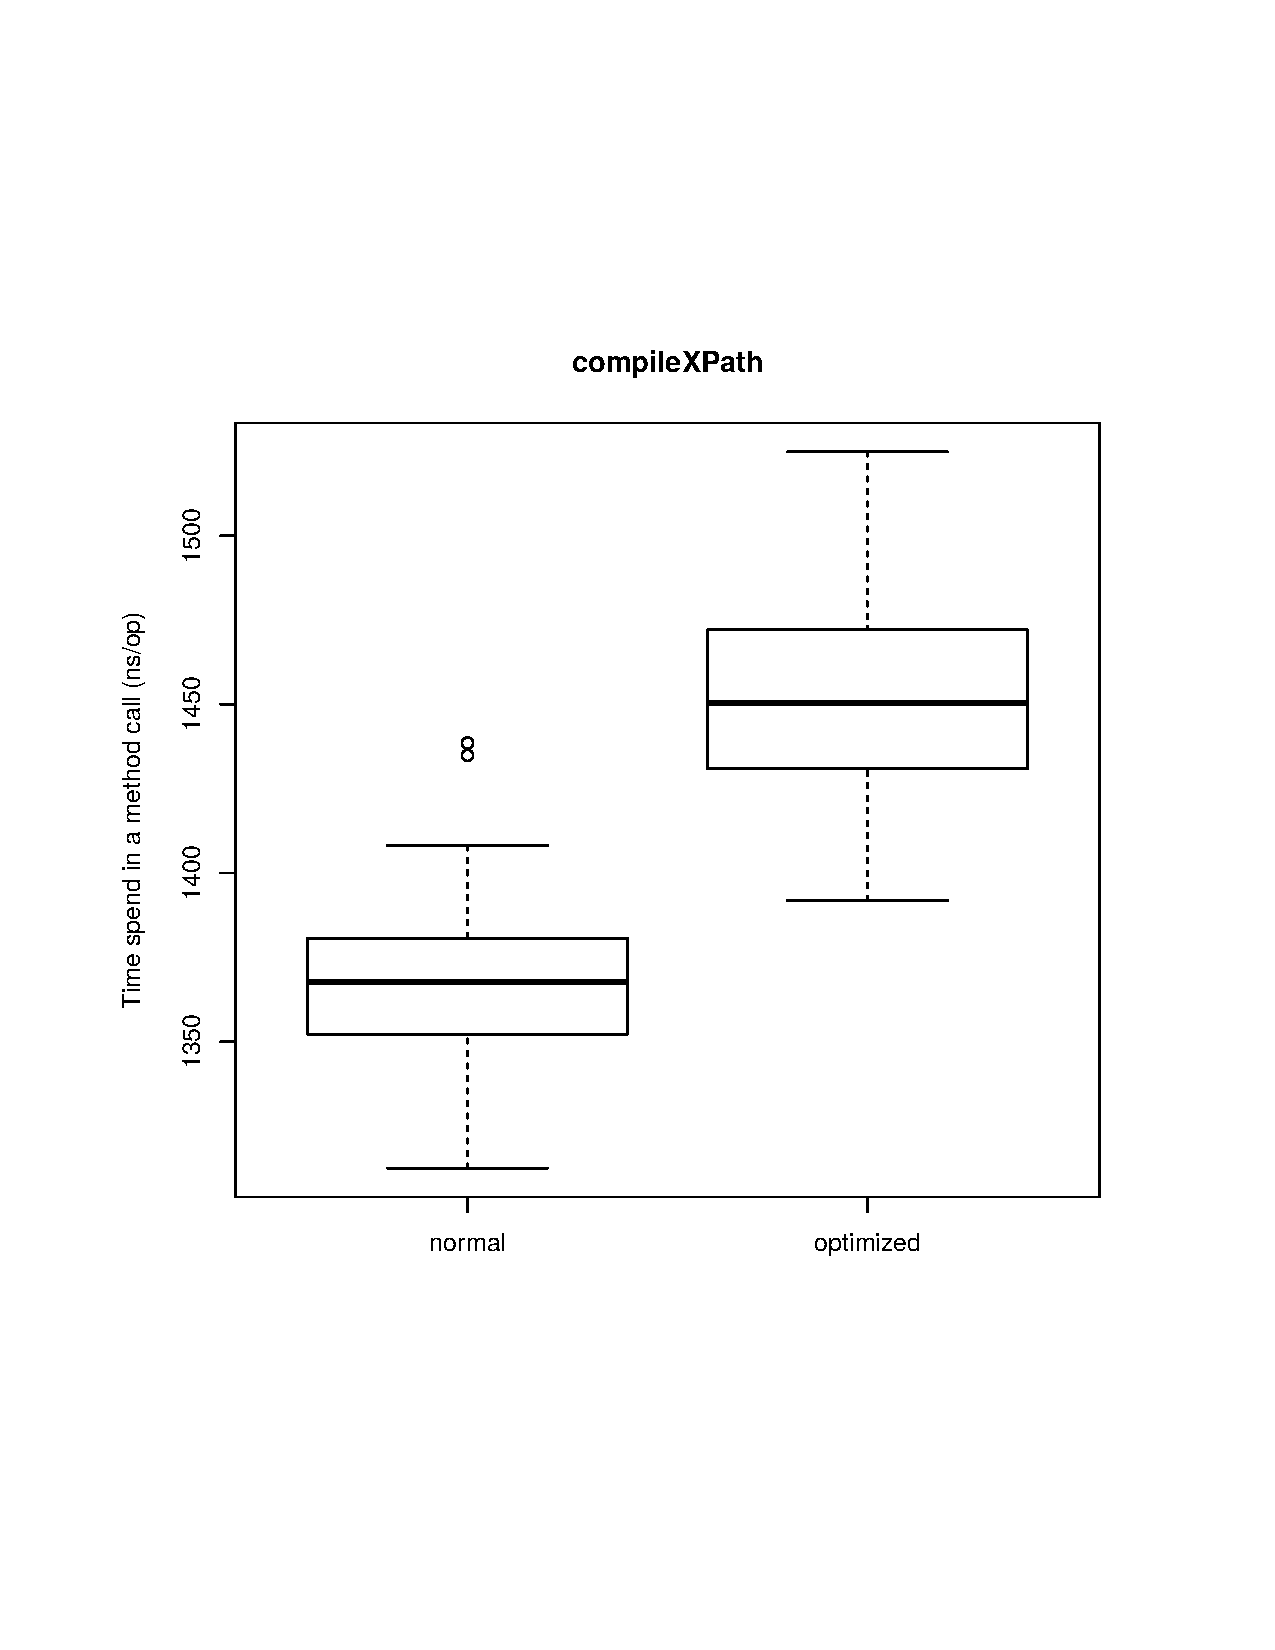
\includegraphics[trim=0mm 60mm 20mm 50mm,scale=0.50]{pictures/boxplot_compileXPath.pdf}
		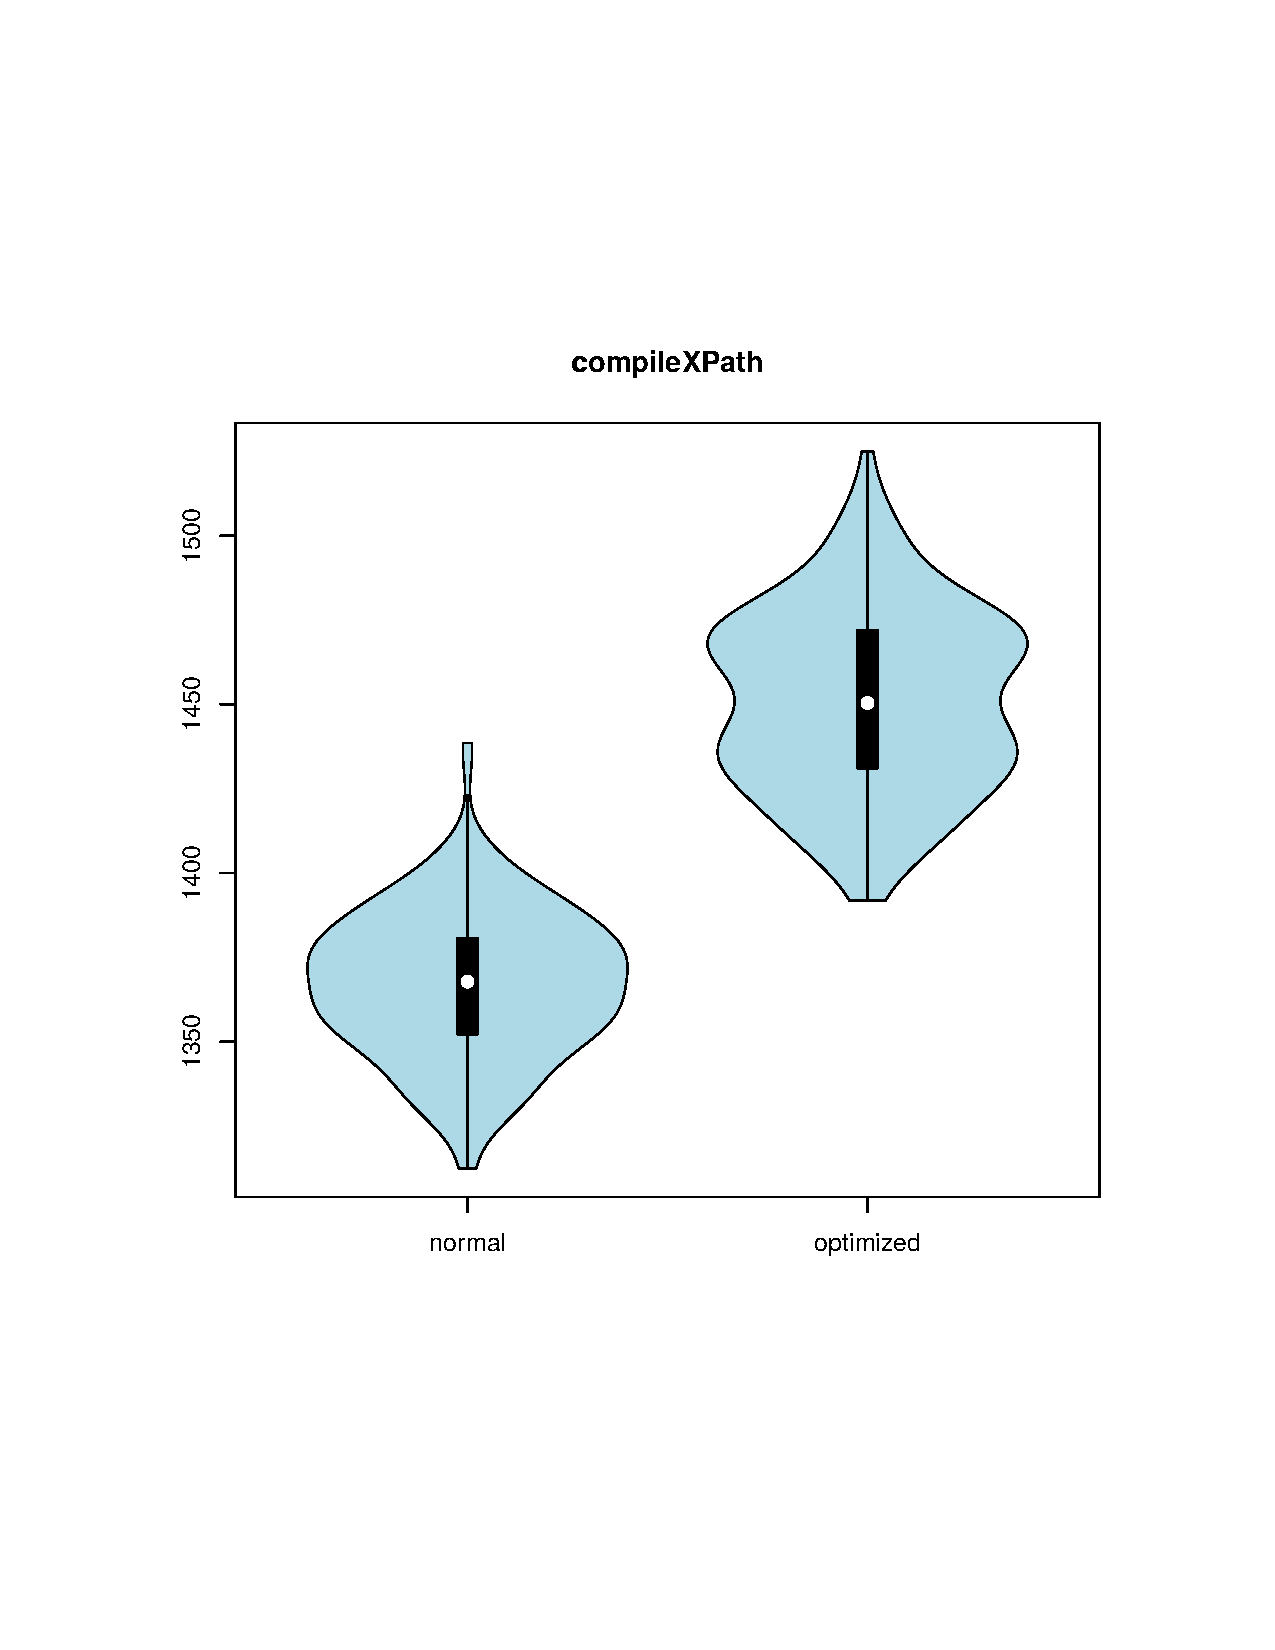
\includegraphics[trim=20mm 60mm 0mm 50mm,scale=0.50]{pictures/vioplot_compileXPath.pdf}
	}

	\begin{table}[H]
	\centering
		\begin{tabular}{|r|r|r|r|}
			\hline
		   	in $ns$ 	  & Mittelwert & Median & \bf{$\pm$ $0,1\%$} \\
		 	\hline
		 	\hline
		  	normal 	  & 1366,91 & 1367,75 & 5,053 \\
		 	optimiert & 1451,09 & 1450,40 & 6,346 \\ 
		  	\hline
		  	
		\end{tabular}
	\end{table}

	\caption{Ergebnis des XPath Compile Benchmarks}\label{bp:compile}
\end{figure}

\paragraph{Auswertung}

Die \texttt{tokenize} Methode ist im Gegensatz zu den bisher betrachteten optimierten Methoden deutlich
komplexer. Die einzelnen im String gefunden Token werden einer sogenannte \textit{Token-Queue} 
hinzugefügt. Dies geschieht über die private Methode \texttt{addToTokenQueue}. Dabei 
werden bei jedem dieser Aufrufe das Ergebnis eines \texttt{substring} Aufrufs übergeben.

Eine weitere wichtige Methode während des Erzeugung der Token ist die Methode \texttt{mapNSTokens},
welcher der Eingabe String übergeben wird. Innerhalb dieser Methode werden \texttt{substring}  
Aufrufe auf dem übergebenen String ausgeführt.

Abgesehen von der Übergabe als Parameter werden auf den String nur unterstützte Methoden 
ausgeführt:

\begin{itemize}
 	\item \texttt{length()}
 	\item \texttt{charAt(int)}
\end{itemize} 

Bereits die Verwendungen der optimierten Referenzen als Übergabe Parameter zu 
Konvertierungen zurück zum originalen String Typ. Zusätzlich geschehen diese Konvertierungen 
innerhalb einer Schleife, die über alle \texttt{char}s
des String läuft. Daher führen die Konvertierungen in dieser Methode zu einer 
erheblichen Zunahme der Laufzeit.  
